\chapter{Results and Comparisons} 
\label{ch:results} 
\section{Test Case 1}
The results for Test Case 1 in each model are depicted in \figurename~\ref{figure_testcase1}. Both models exhibited similar outcomes, revealing a fundamental vibration frequency of 0.43 Hz. The maximum bit velocity was at 79 RPM for the A-S model and 81 RPM for the ExxonMobil model. Also, the torque on the top drive was predicted as 1762 lb-ft for the A-S model and 1814 lb-ft for the ExxonMobil model. The comparison between the results from different models are illustrated in \figurename~\ref{figure_testcase1_overlapped}. Although both models exhibited similar frequencies, the minimal phase differences (1e3$^{\circ}$ ) contribute to the observed shift between the two models.
\begin{figure}
  \centering
  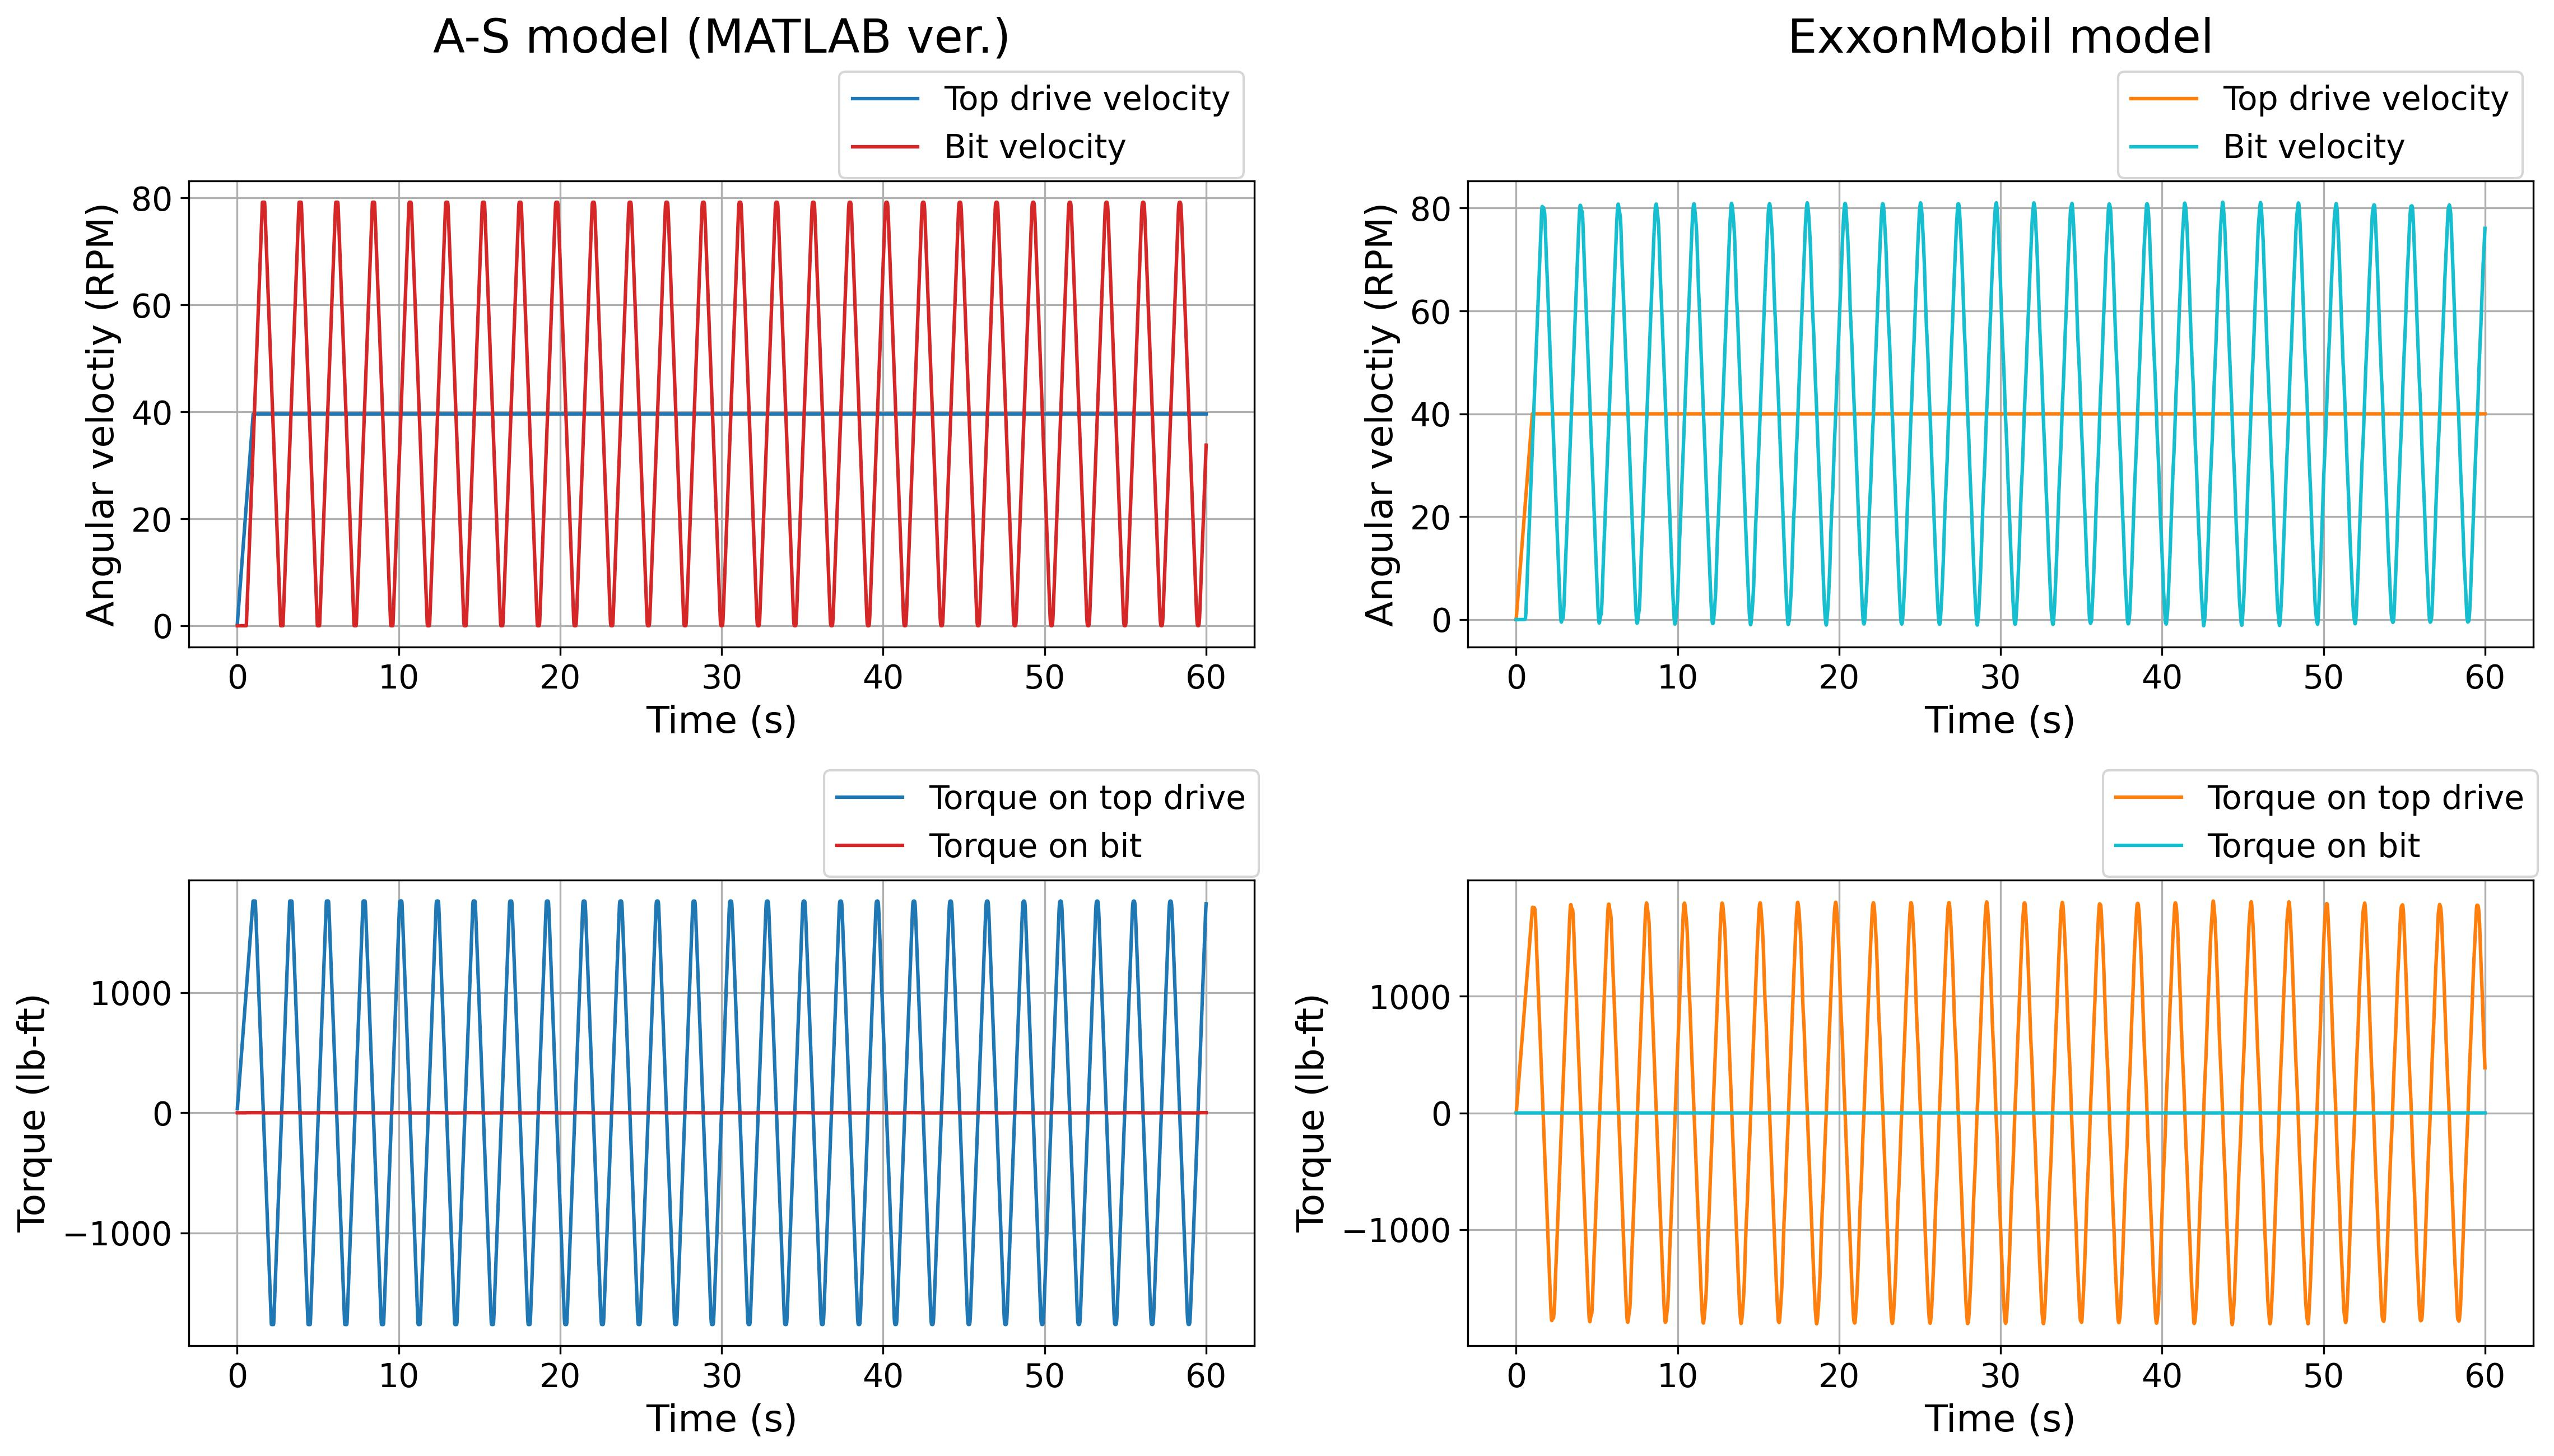
\includegraphics[width=6.5in]{output_figureTestCase1}
  \caption[Results of Test Case 1]{Results of Test Case 1. First and second columns show the results from A-S model (MATLAB ver.) and ExxonMobil model, respectively.}\label{figure_testcase1}
\end{figure}

\begin{figure}
  \centering
  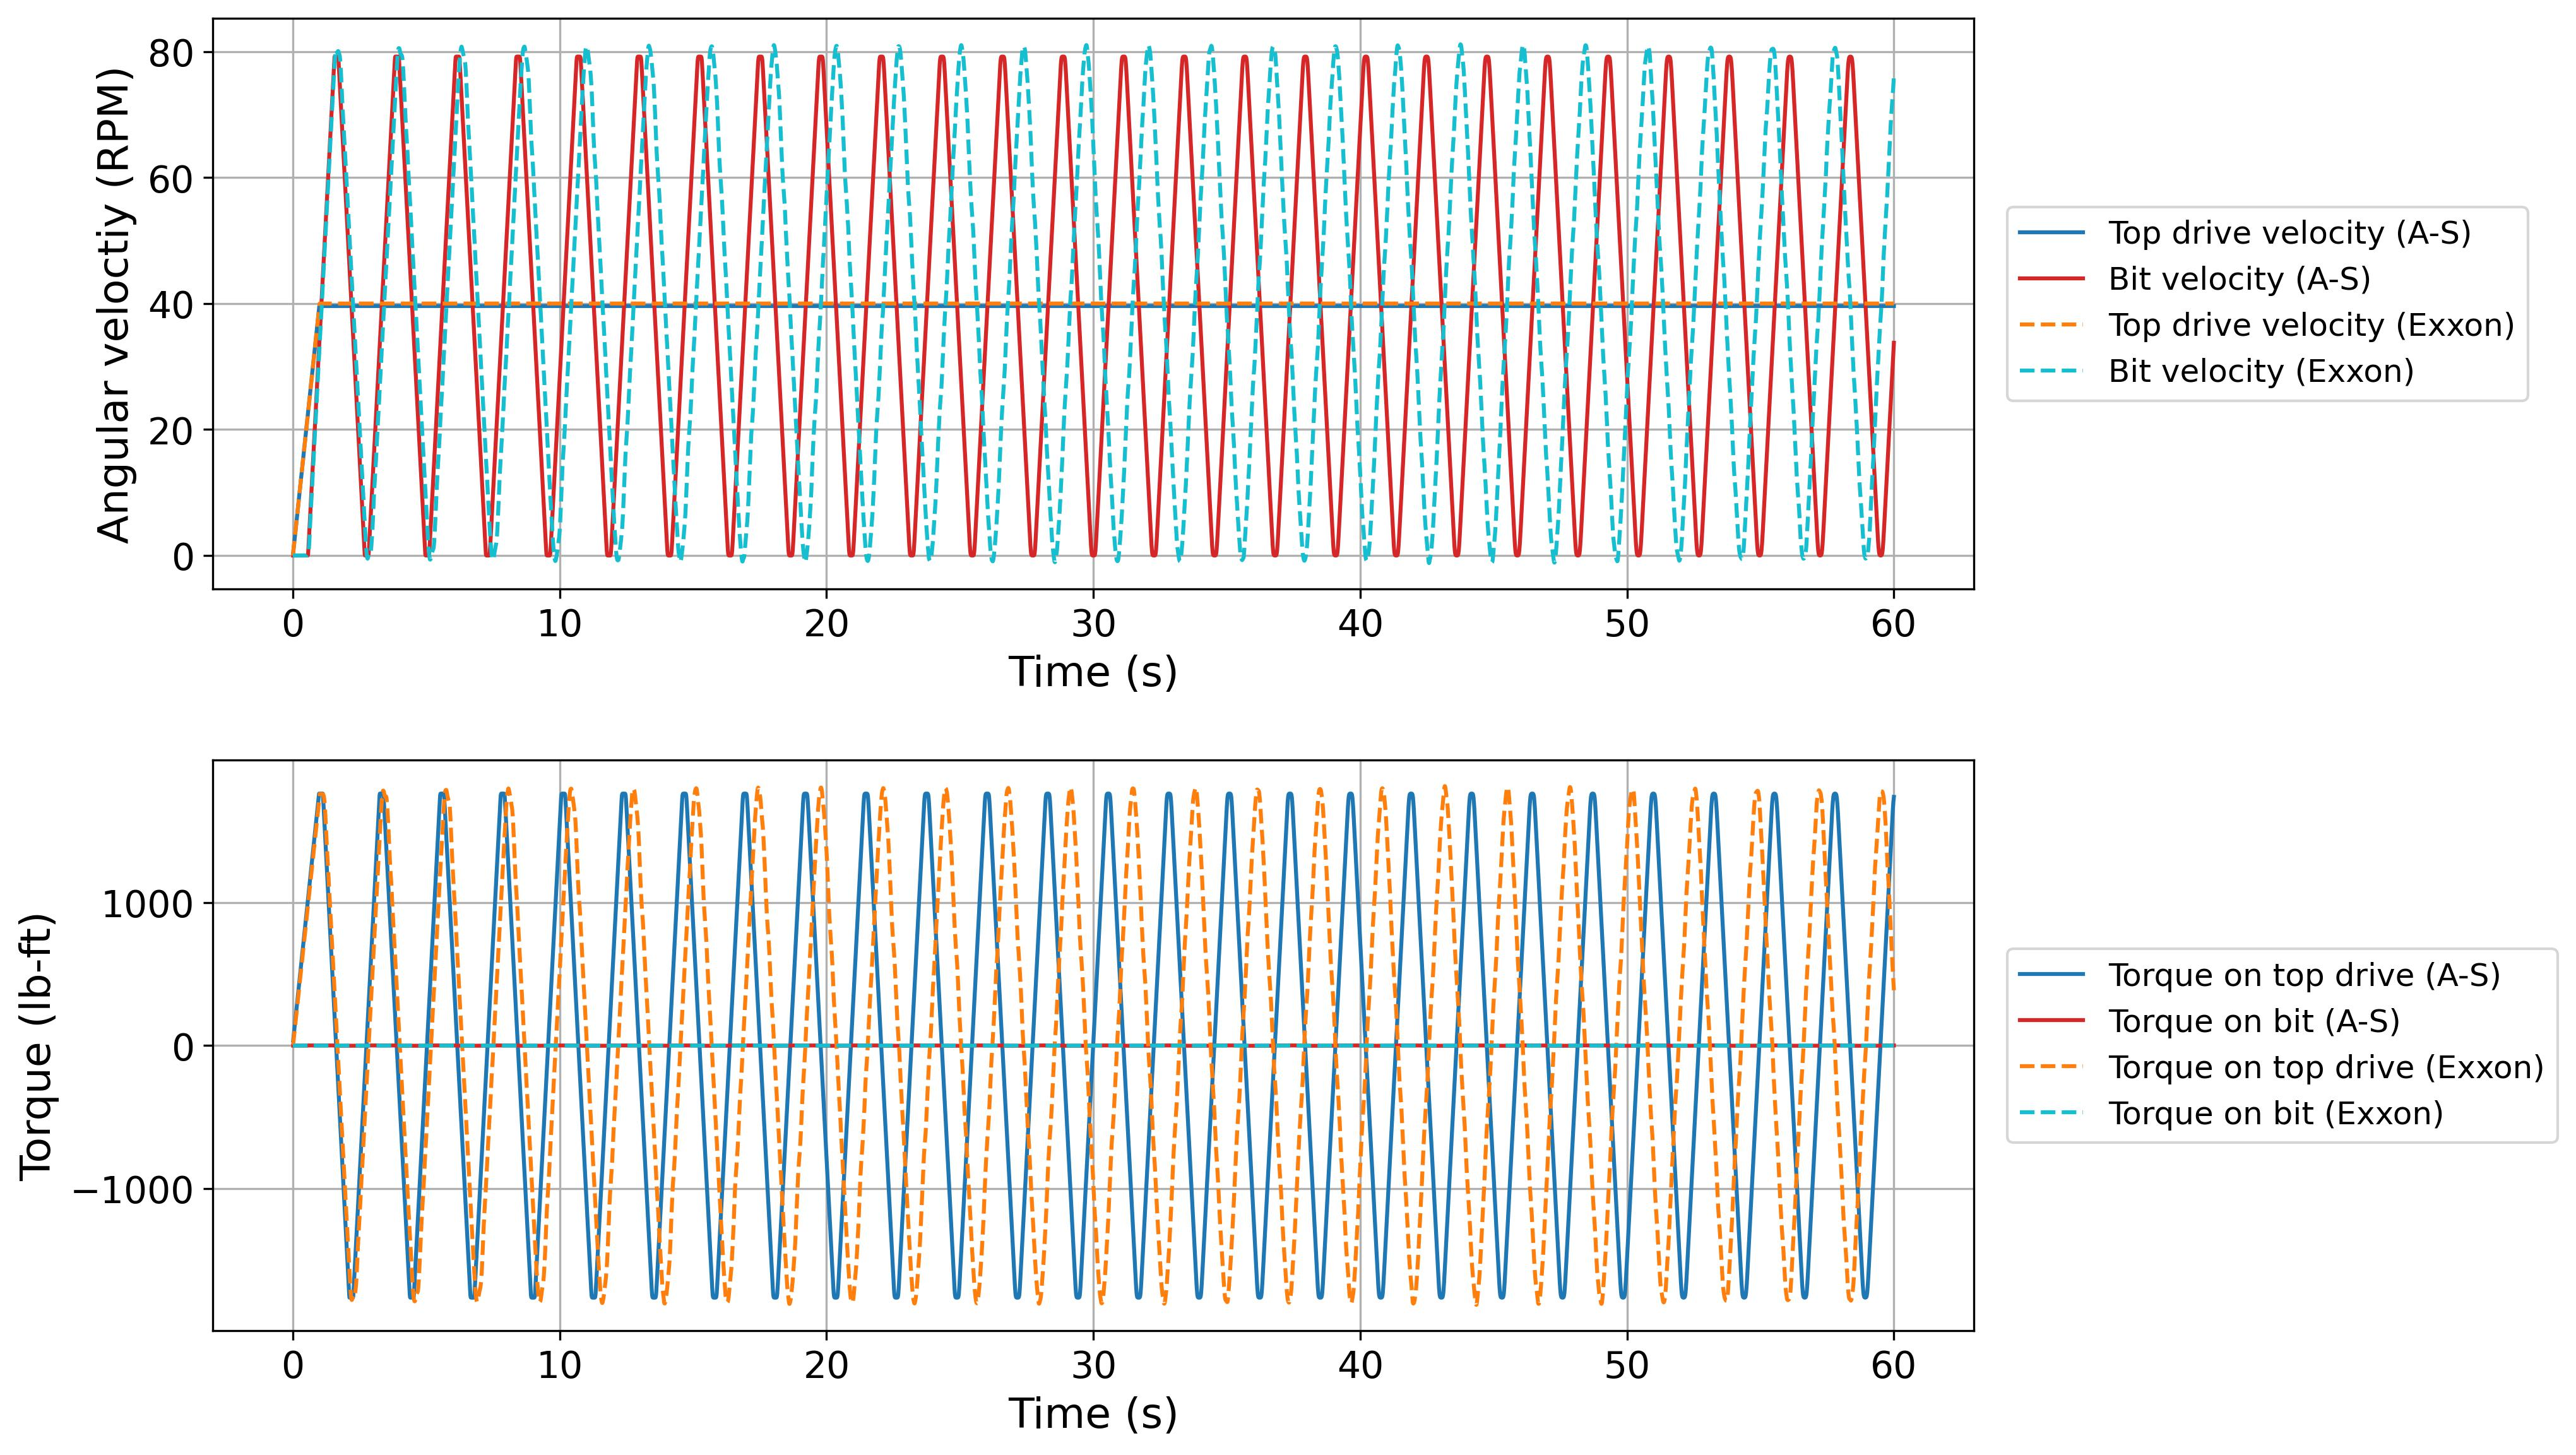
\includegraphics[width=6.5in]{overlapped_figureTestCase1}
  \caption[Comparison of the results for Test Case 1]{Comparison between the results from A-S model (MATLAB ver.) and ExxonMobil model for Test Case 1.}\label{figure_testcase1_overlapped}
\end{figure}

\section{Test Case 2}
\subsection{Test Case 2a}
The results for Test case 2a from each model are depicted in \figurename~\ref{figure_testcase2_1}. Similar to Test case 1, both model well matched with fundamental vibration frequencies of 0.28 and 0.27 for A-S model and ExxonMobil model, respectively. The maximum bit velocity was at 78 RPM for the A-S model and 79 RPM for the ExxonMobil model, while the torque on the top drive was predicted as 6643 lb-ft for the A-S model and 6891 lb-ft for the ExxonMobil model. \figurename~\ref{figure_testcase2_1_overlapped} illustrates the comparison of the results from two different models. 
\begin{figure}
  \centering
  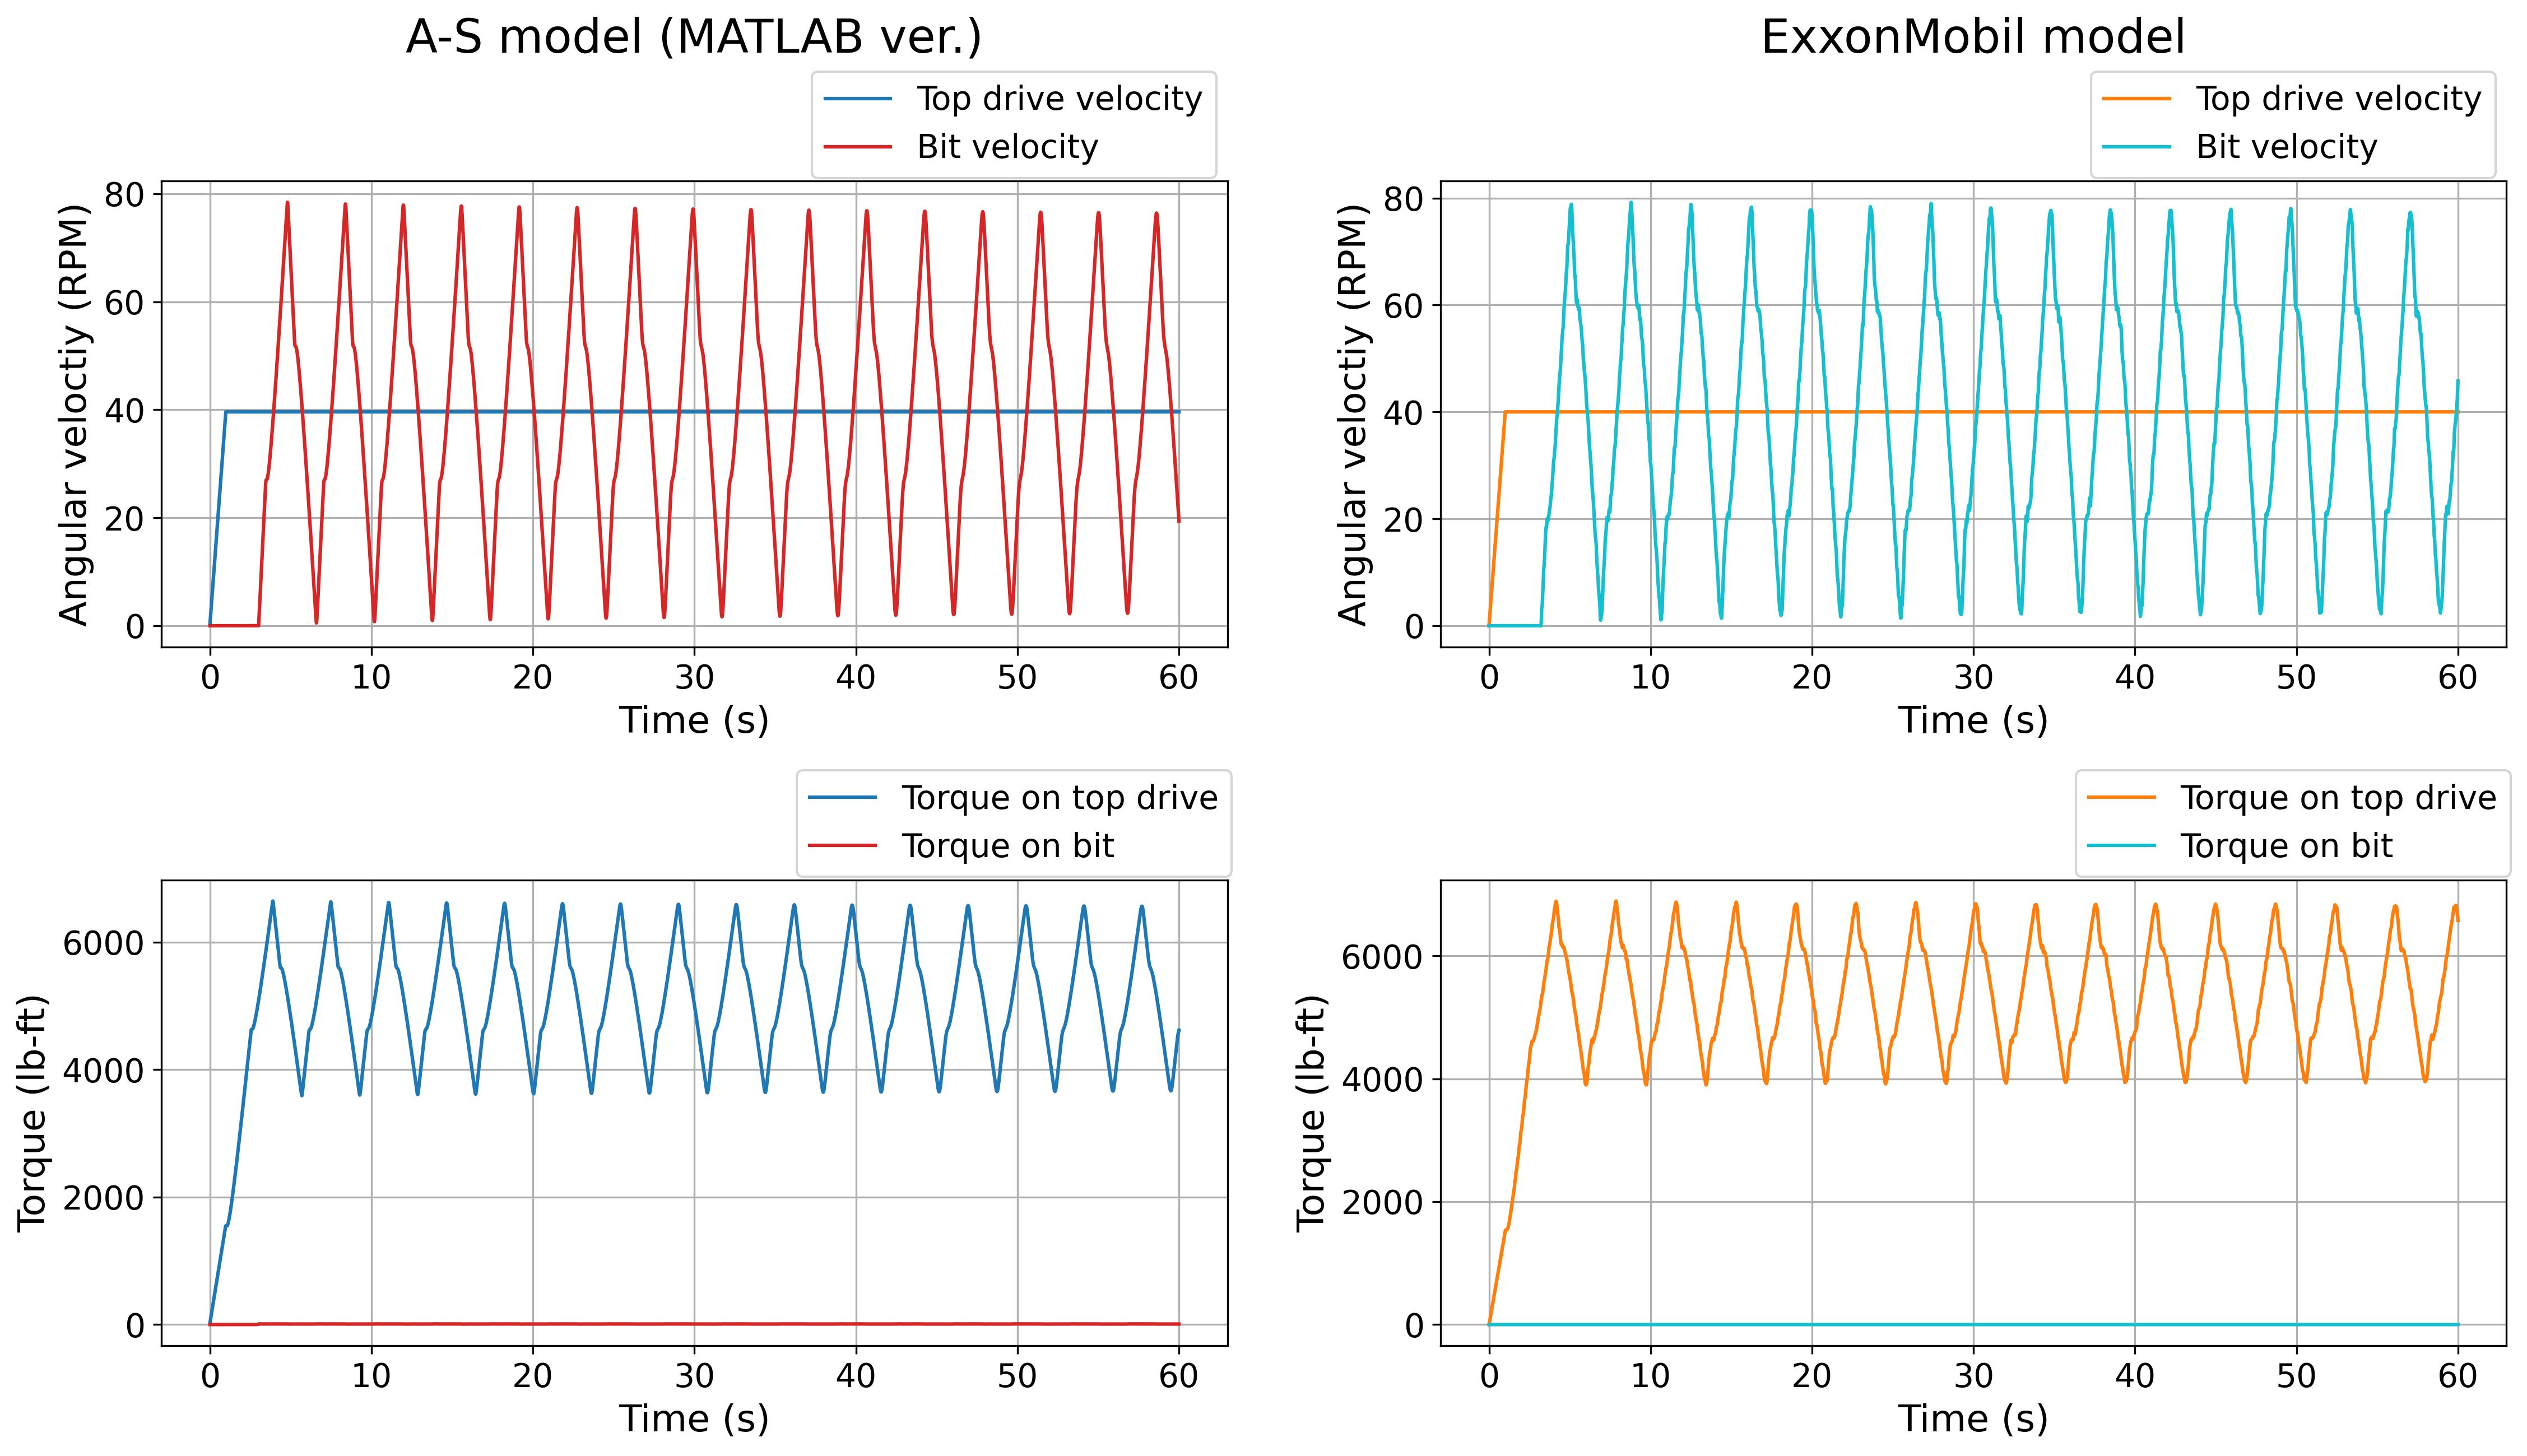
\includegraphics[width=6.5in]{output_figureTestCase2_1}
  \caption[Results of Test Case 2a]{Results of Test Case 2a. First and second columns show the results from A-S model (MATLAB ver./) and ExxonMobil model, respectively.}\label{figure_testcase2_1}
\end{figure}

\begin{figure}
  \centering
  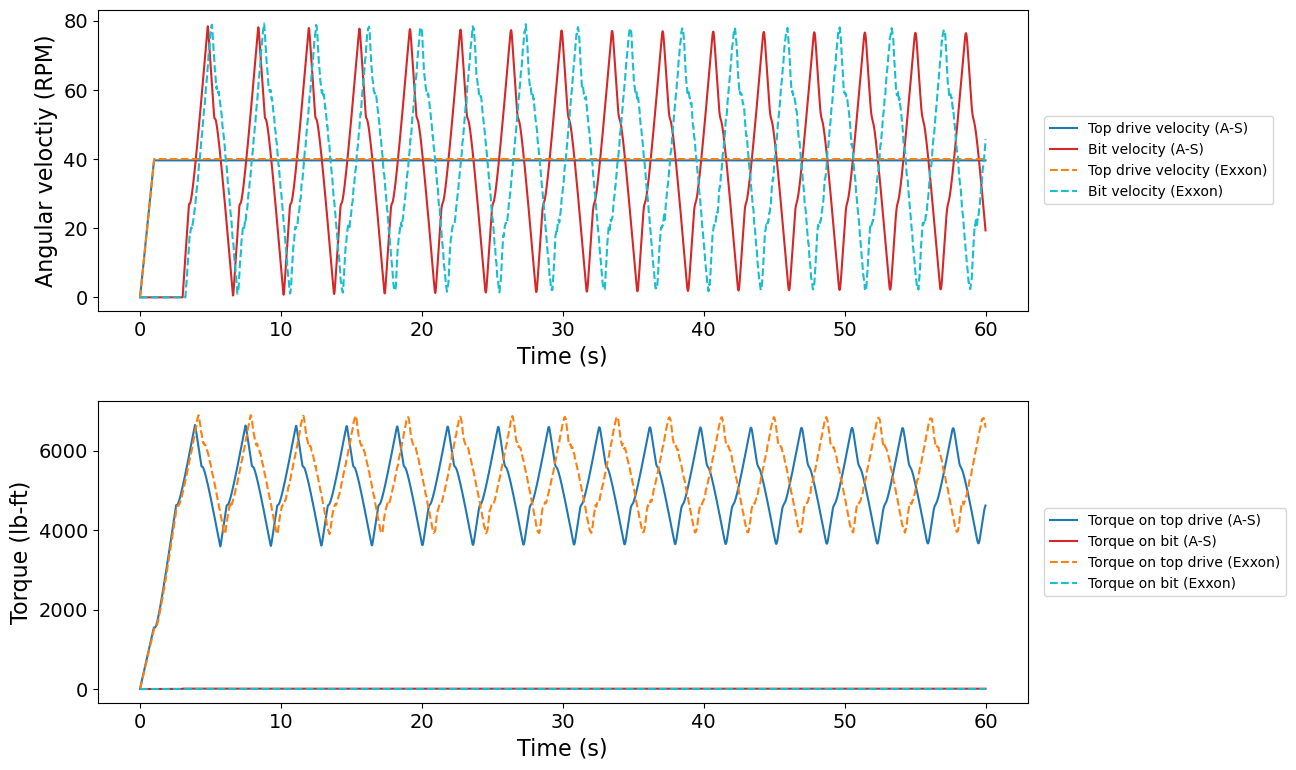
\includegraphics[width=6.5in]{overlapped_figureTestCase2_1}
  \caption{}\label{figure_testcase2_1_overlapped}
\end{figure}


\subsection{Test Case 2b}
The results for Test case 2b from each model are depicted in \figurename~\ref{figure_testcase2_2}. The stick-slip behavior during drilling was observed in both models, which is about 2 seconds of stick phase. This event was caused by Coulomb friction from well deviated well. This reveals the effect of the dynamic friction factor on the drilling dysfunction since only dynamic friction is reduced to half in Test case 2b compared to Test case 2a. Both models showed a spike in bit angular velocity which goes below zero. This has not been investigated yet, but the causation of it can be analyzed in future studies. The transient behavior was observed until around 35 s steady-state behavior was observed after that in both models. However, high amplitude during the transient state was observed in A-S model for both the angular velocity of bit and torque on top drive. 

The fundamental frequencies of the vibration were 0.28 and 0.27 for A-S model and ExxonMobil model, respectively, which is the same as Test case 2a. The maximum bit velocity was at 107 RPM for the A-S model and 116 RPM for the ExxonMobil model, respectively, while the torque on the top drive was predicted as 5185 lb-ft for the A-S model and 5540 lb-ft for the ExxonMobil model, where the maximum values occurred at the first cycle. \figurename~\ref{figure_testcase2_2_overlapped} illustrates the comparison of the results from two different models during 60 seconds of modeling. Relatively similar behavior can be seen from the comparison, and also the effect of the phase shift was observed.

\begin{figure}
  \centering
  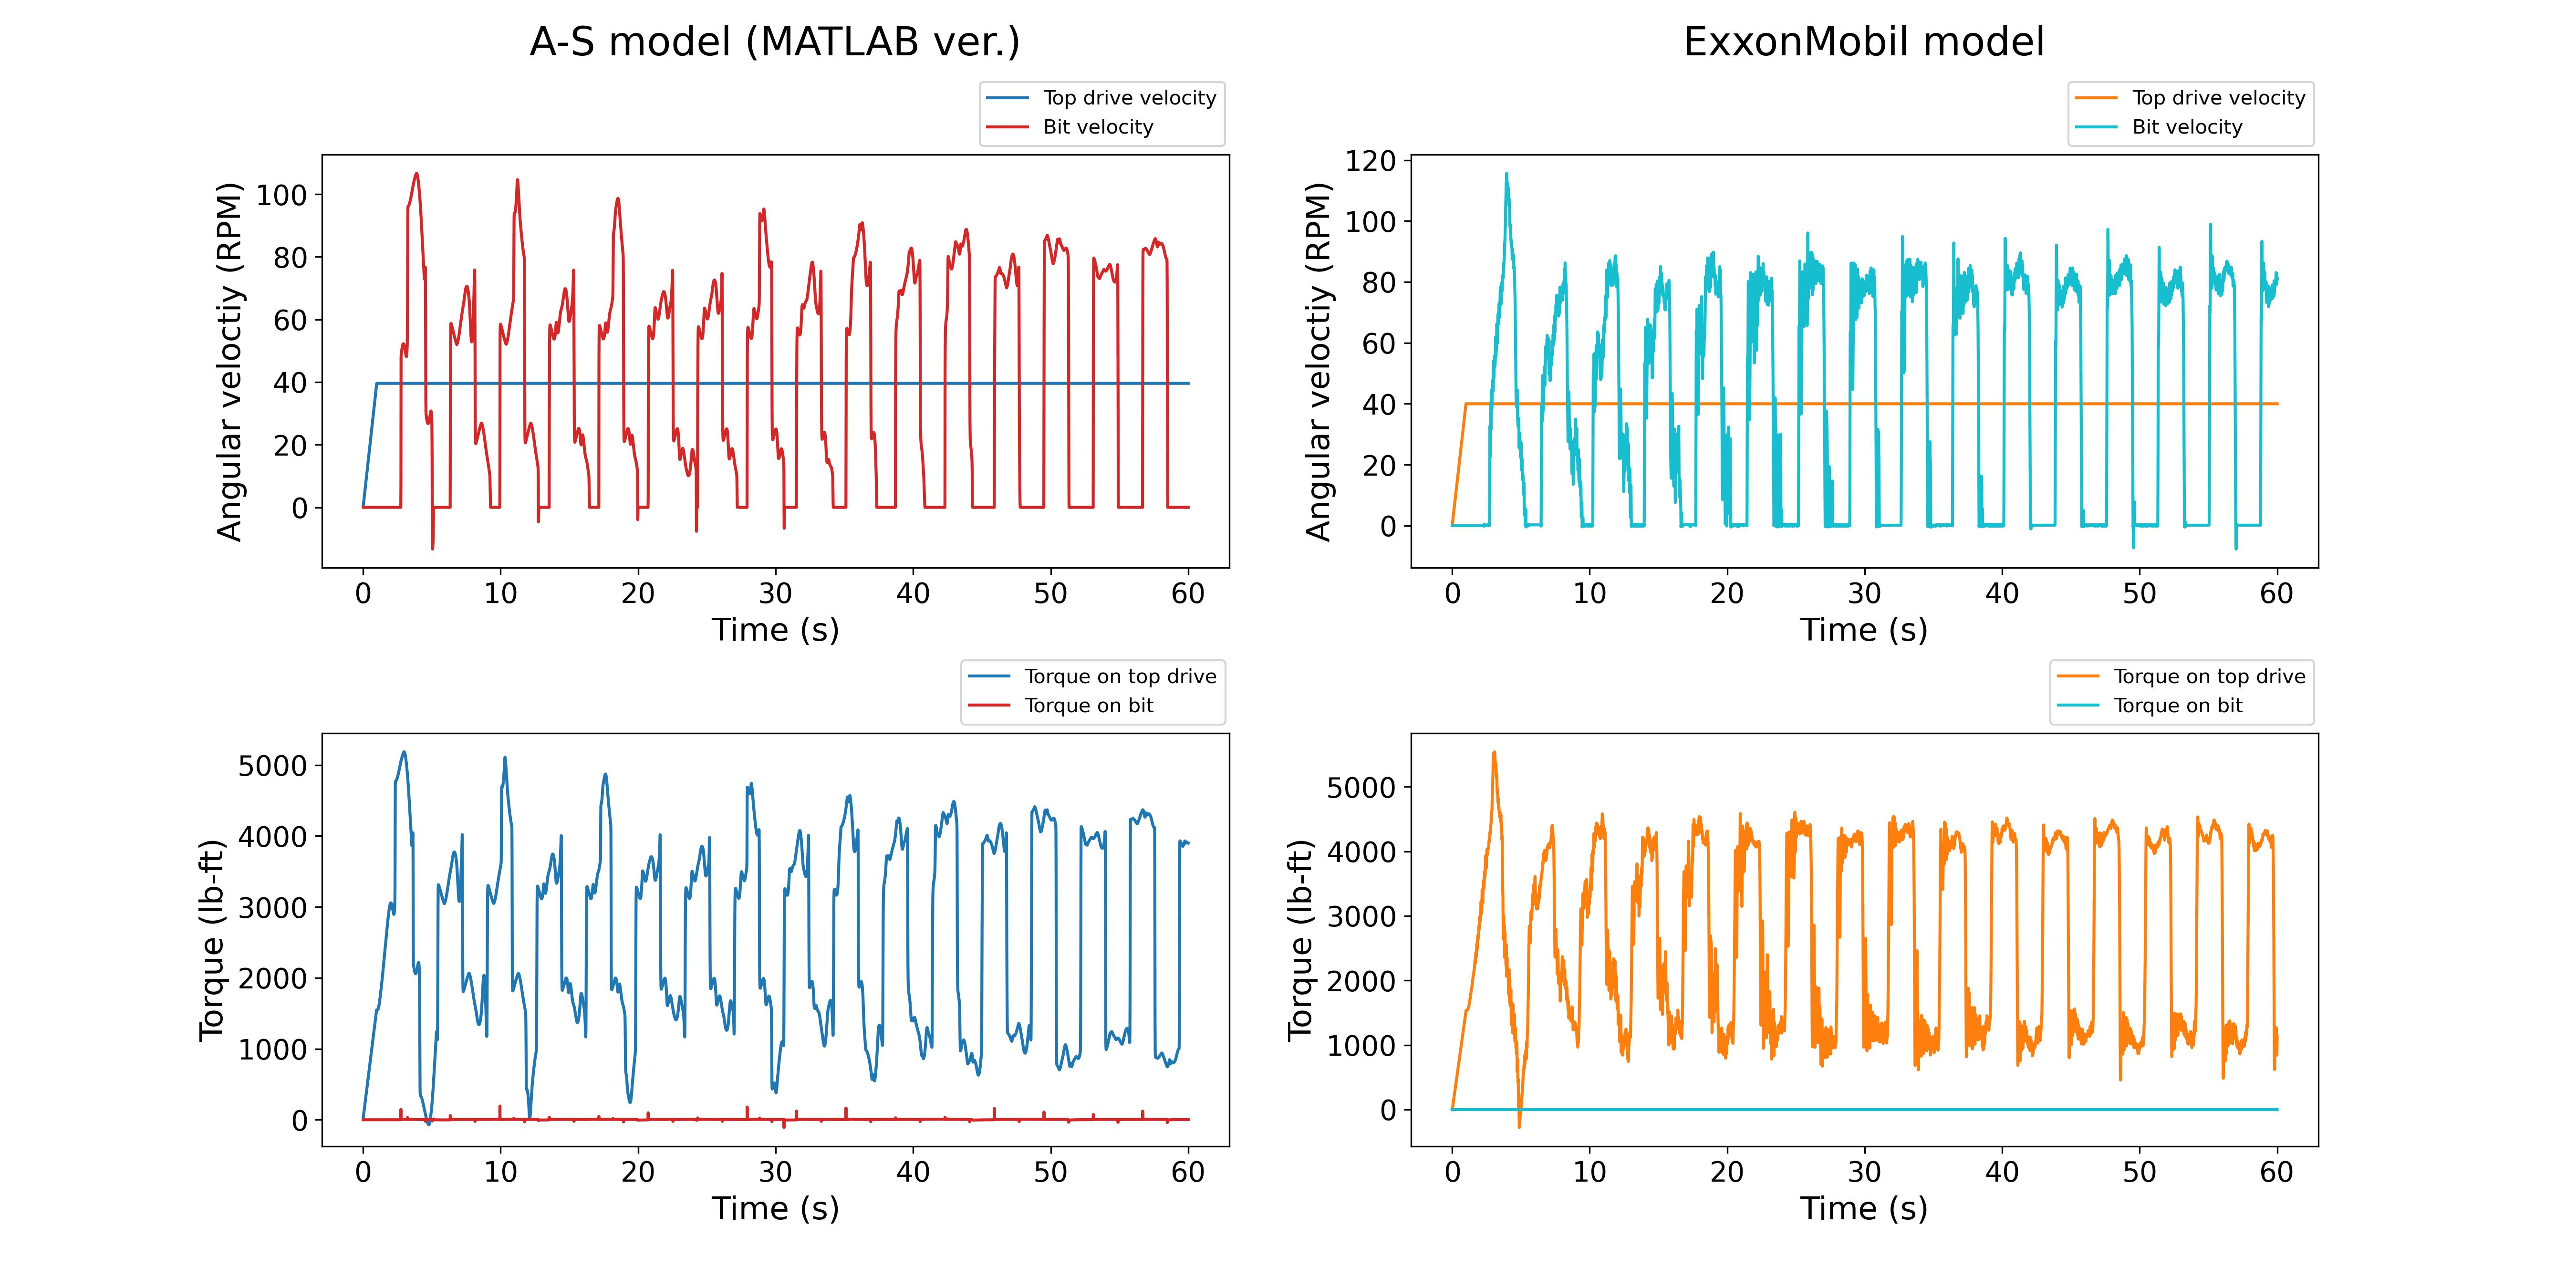
\includegraphics[width=6.5in]{output_figureTestCase2_2}
  \caption{}\label{figure_testcase2_2}
\end{figure}

\begin{figure}
  \centering
  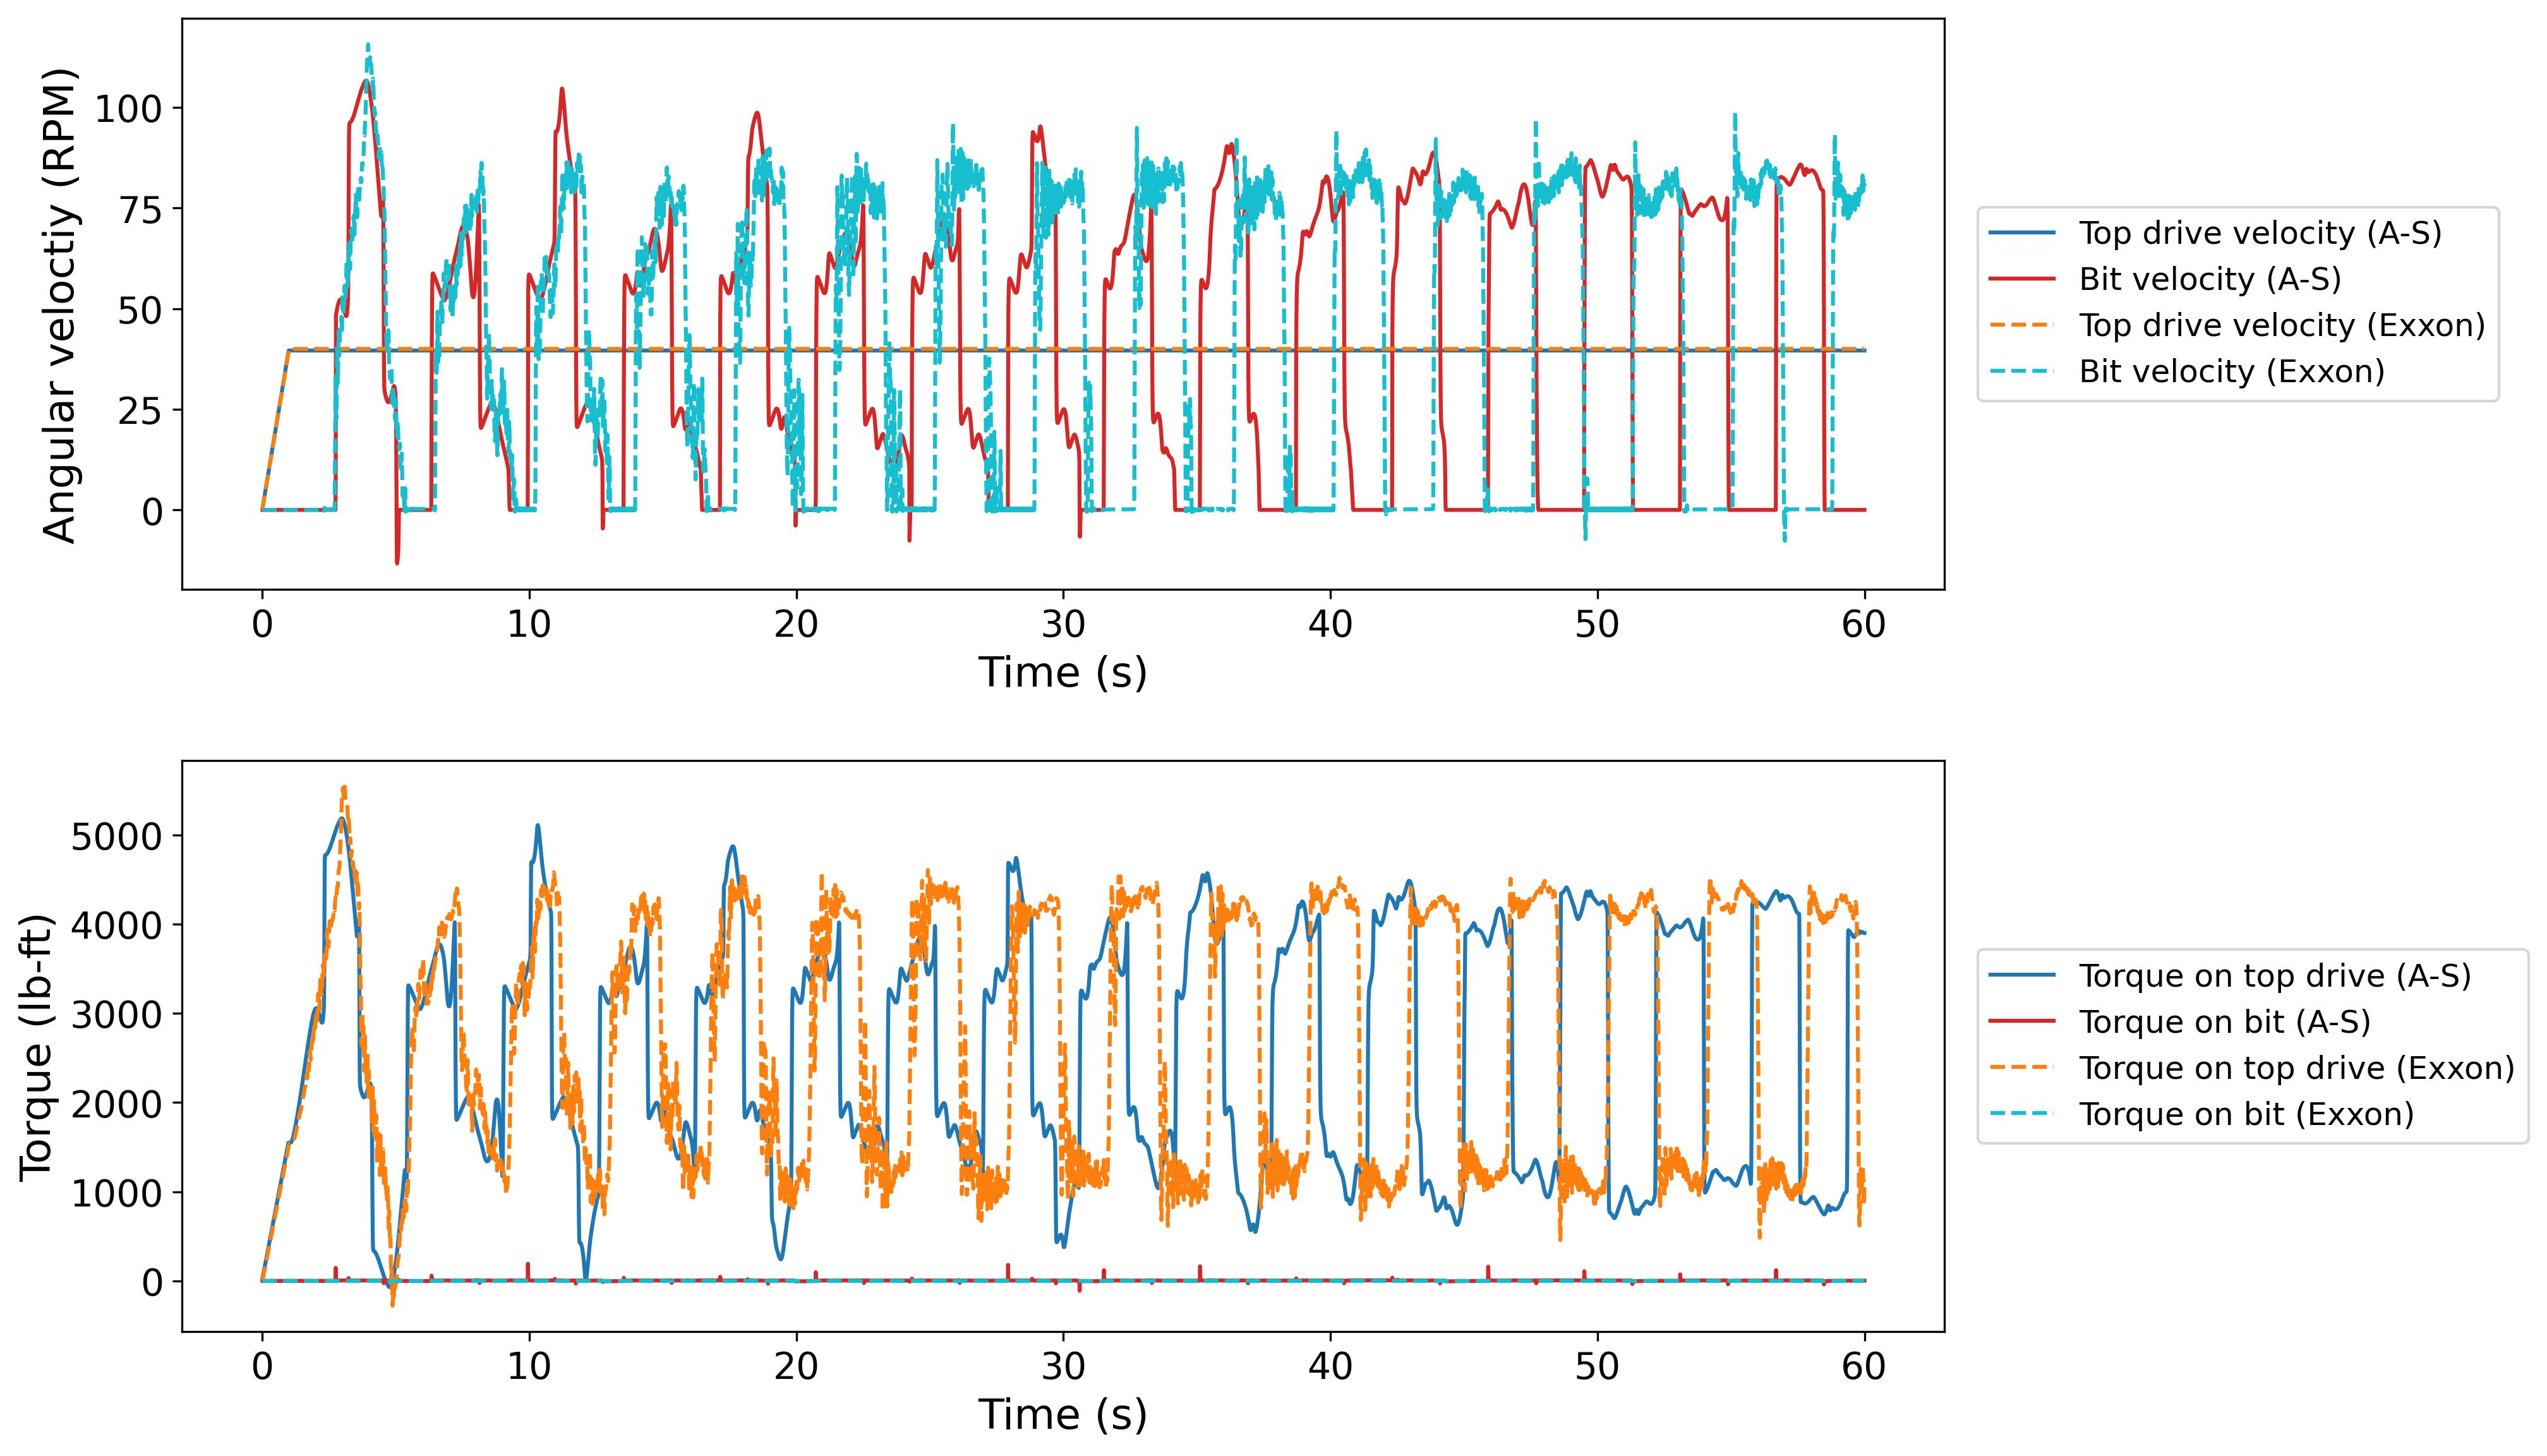
\includegraphics[width=6.5in]{overlapped_figureTestCase2_2}
  \caption{}\label{figure_testcase2_2_overlapped}
\end{figure}

\subsection{Test Case 3}
Test Case 3 shows the effect of BHA components in vertical well. The results show similarities with Test Case 1, but fluctuations in the peak vibration value were observed. Specifically, the peak vibration value decreases until 60 seconds and then starts to increase again, ultimately reaching the same value as the beginning at 120 seconds. Figure \ref{figure_testcase3} and Figure \ref{figure_testcase3_overlapped} illustrate the results for each model and provide comparisons for Test Case 3.

Compared to Test Case 1 (without BHA components), the fundamental vibration frequencies in Test Case 3 were slightly decreased, measuring 0.42 Hz for the A-S model and 0.40 Hz for the ExxonMobil model. Conversely, the bit velocity and torque on the top drive increased. The maximum bit velocity was 80 RPM for the A-S model and 81 RPM for the ExxonMobil model, while the torque on the top drive was predicted as 1844 lb-ft for the A-S model and 1841 lb-ft for the ExxonMobil model. Figure \ref{figure_testcase2_1_overlapped} shows the comparison of the results from the two different models.

\begin{figure}
  \centering
  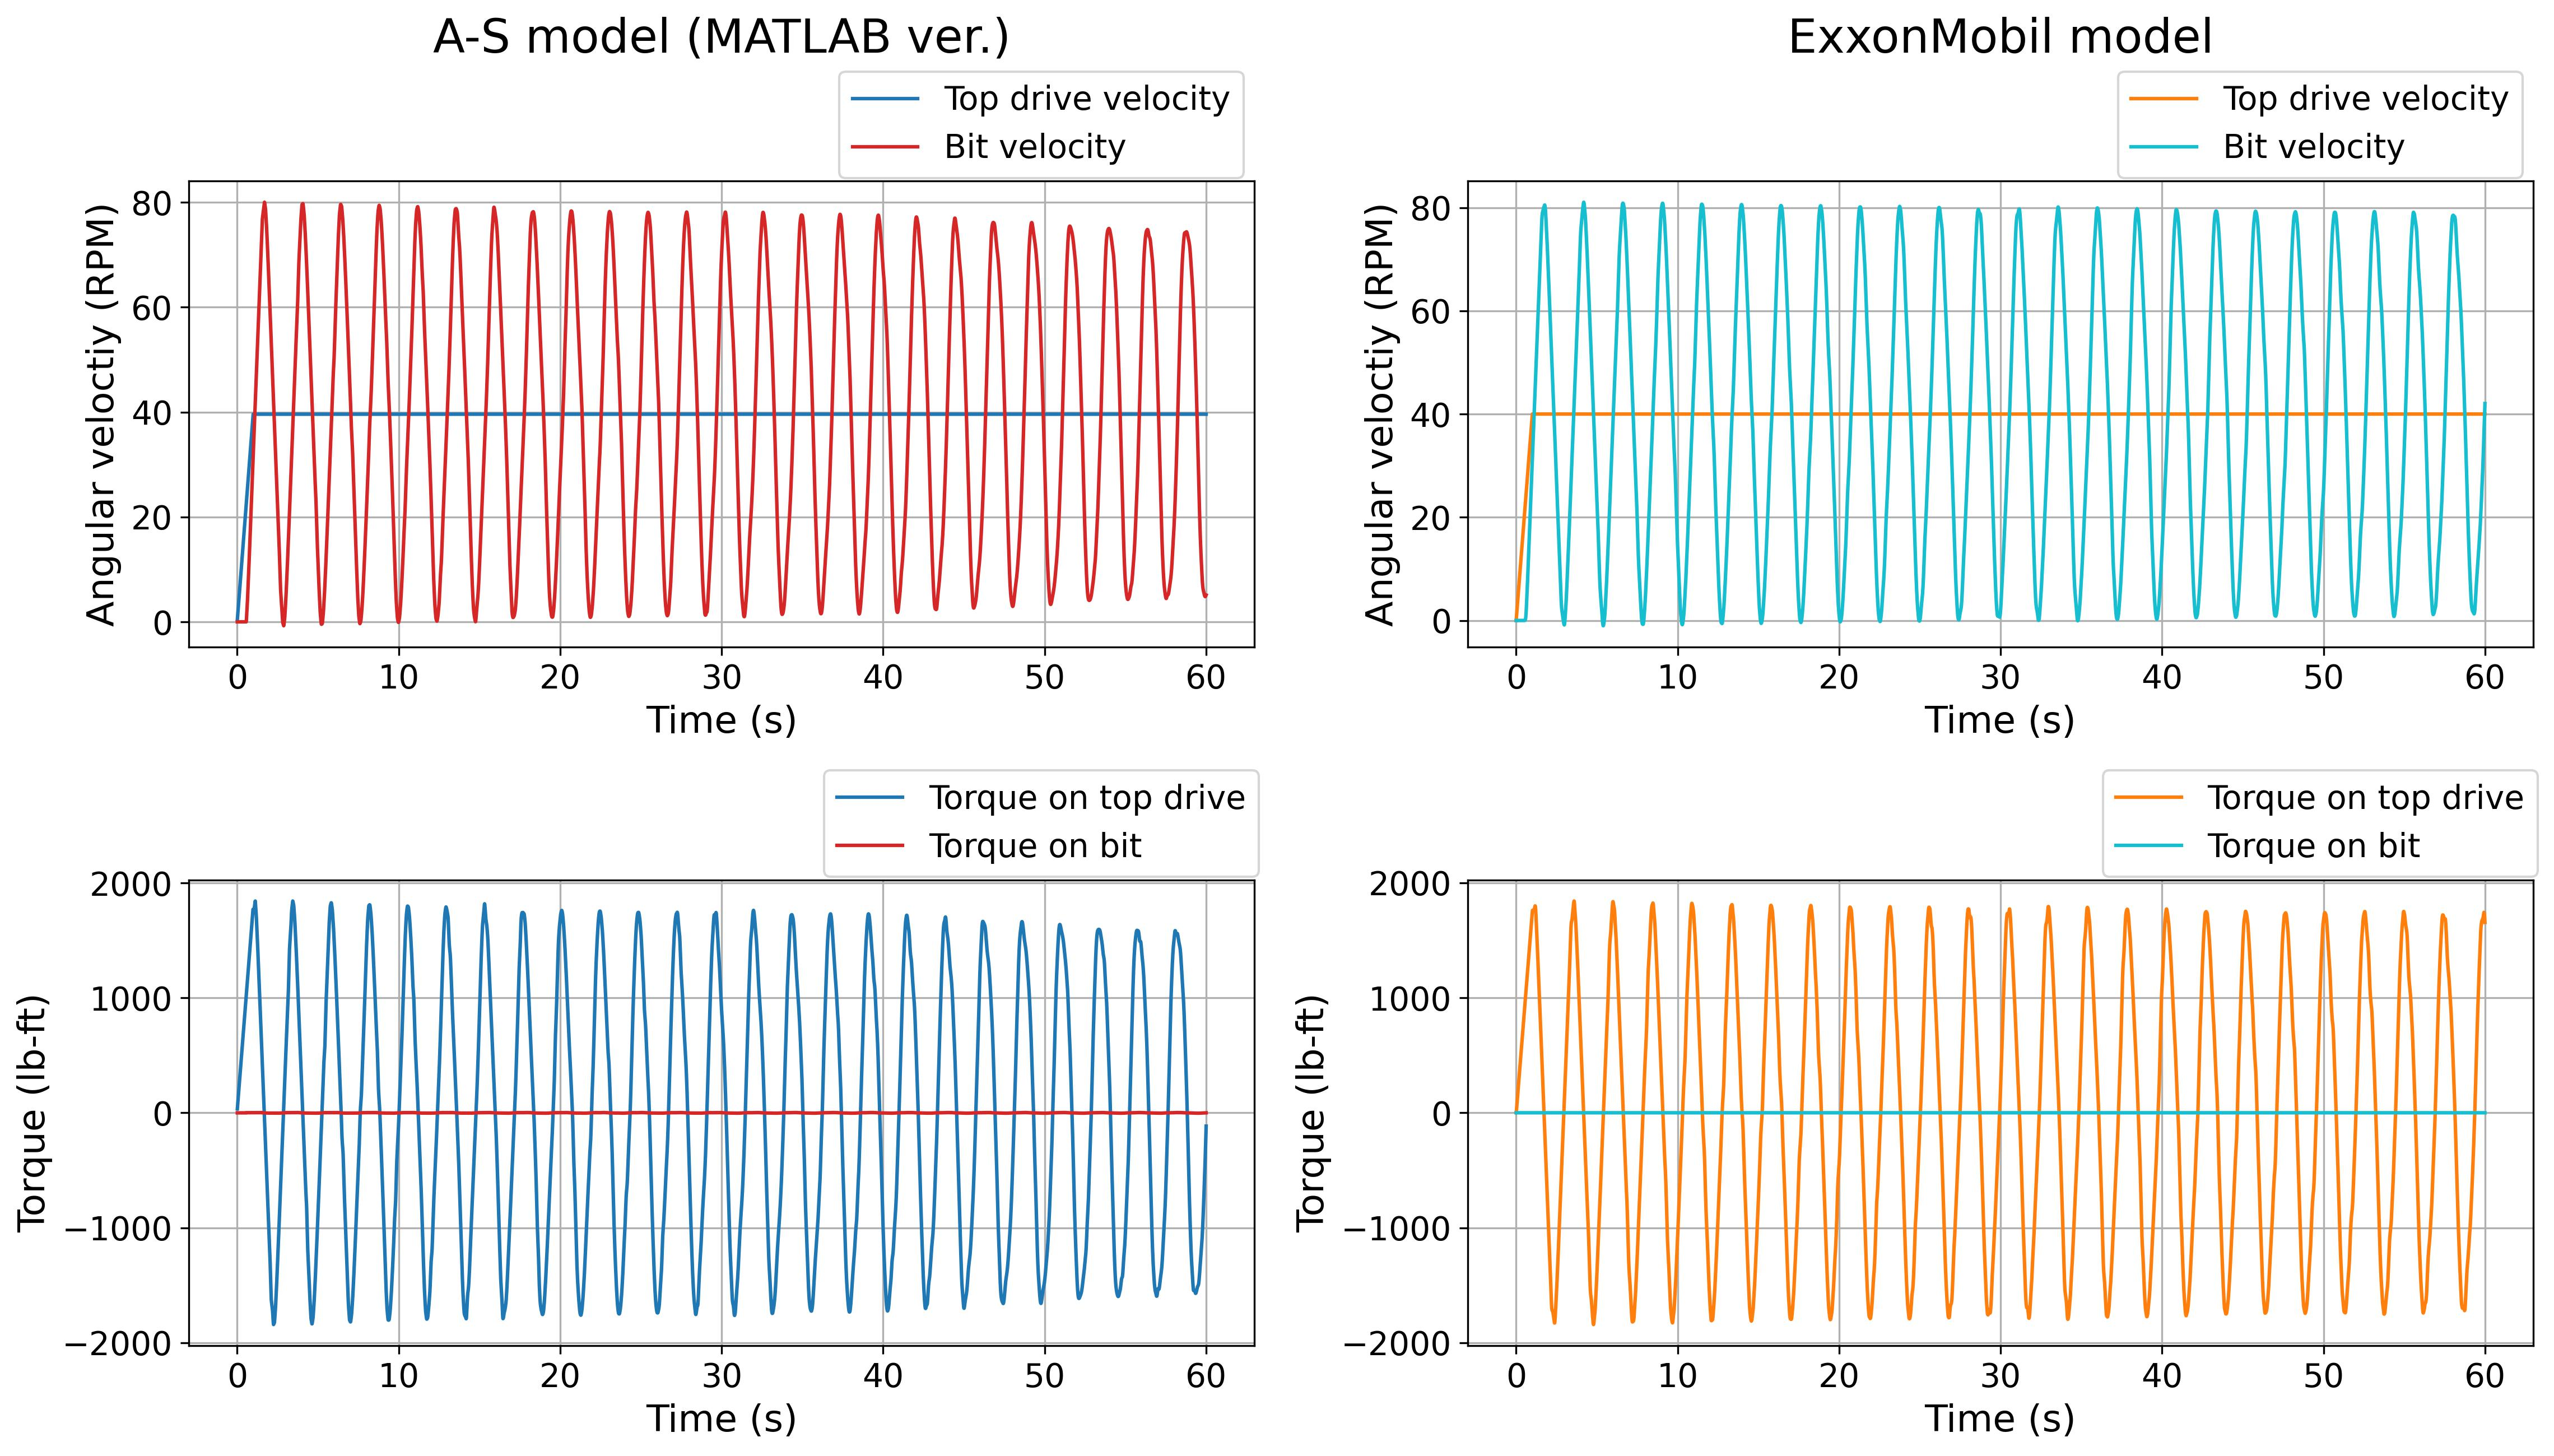
\includegraphics[width=6.5in]{output_figureTestCase3}
  \caption{}\label{figure_testcase3}
\end{figure}
\begin{figure}
  \centering
  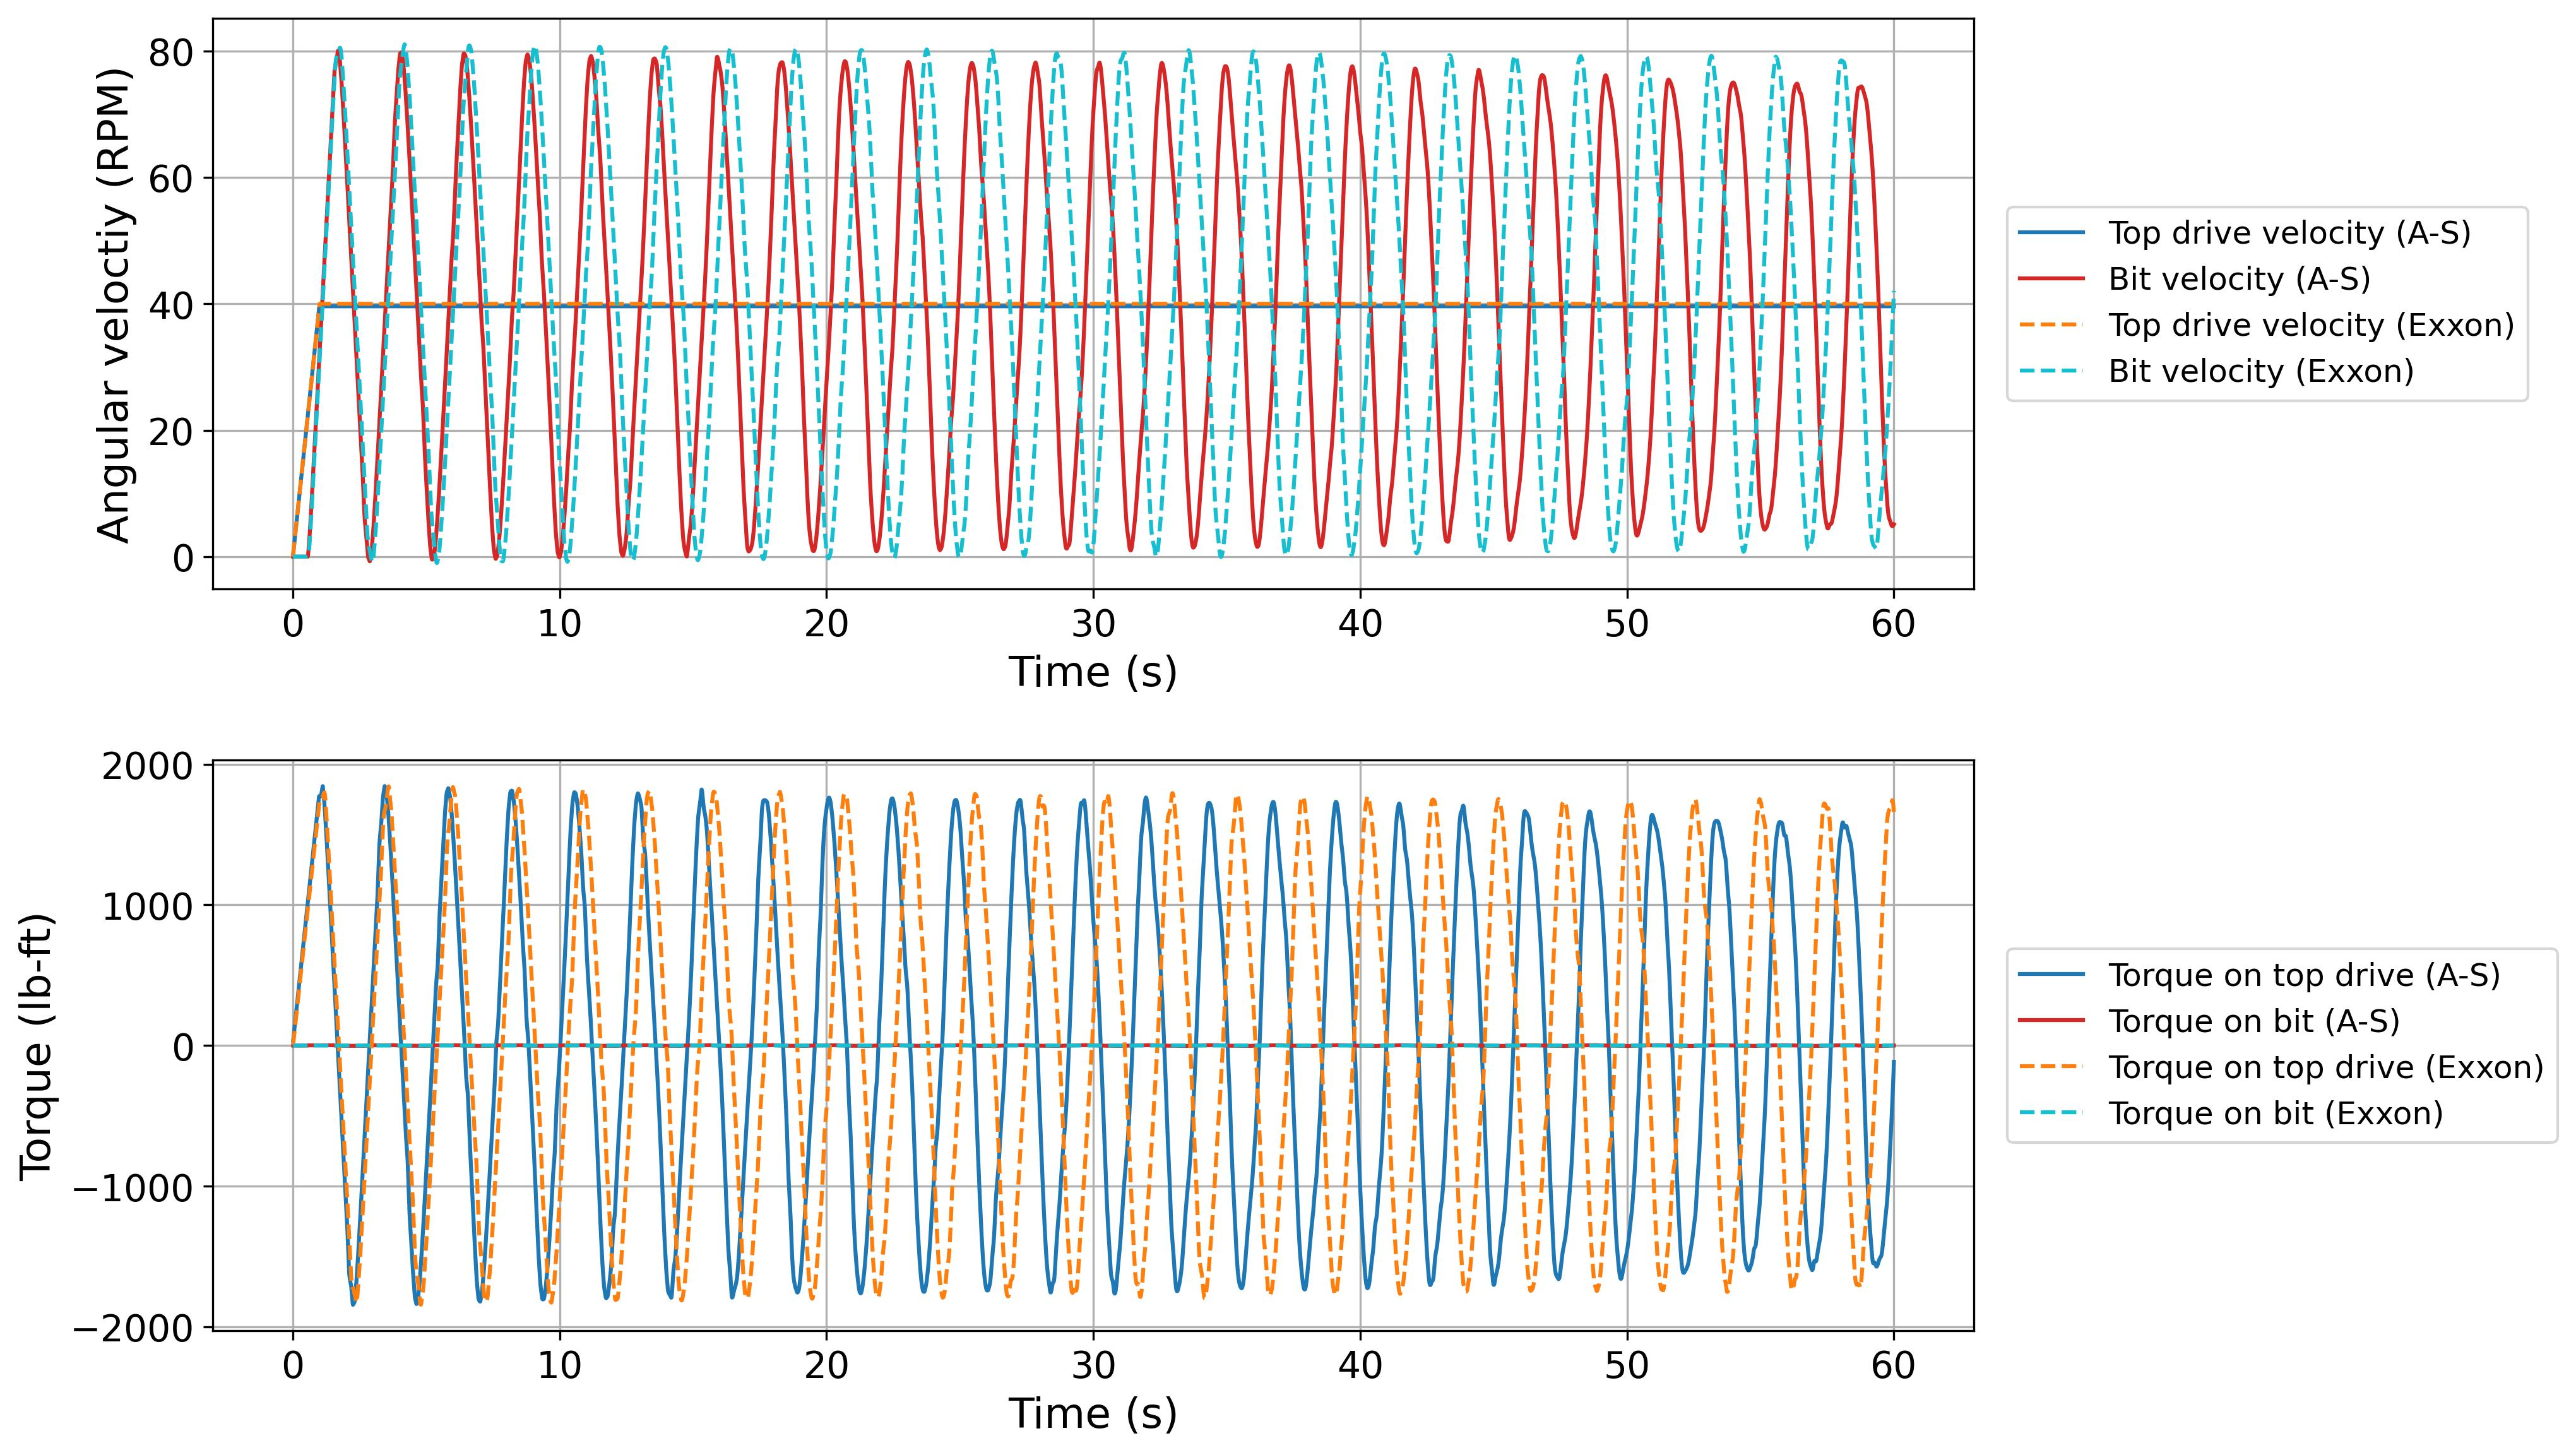
\includegraphics[width=6.5in]{overlapped_figureTestCase3}
  \caption{}\label{figure_testcase3_overlapped}
\end{figure}

\section{Test Case 4}
\subsection{Test Case 4a}
\begin{figure}
  \centering
  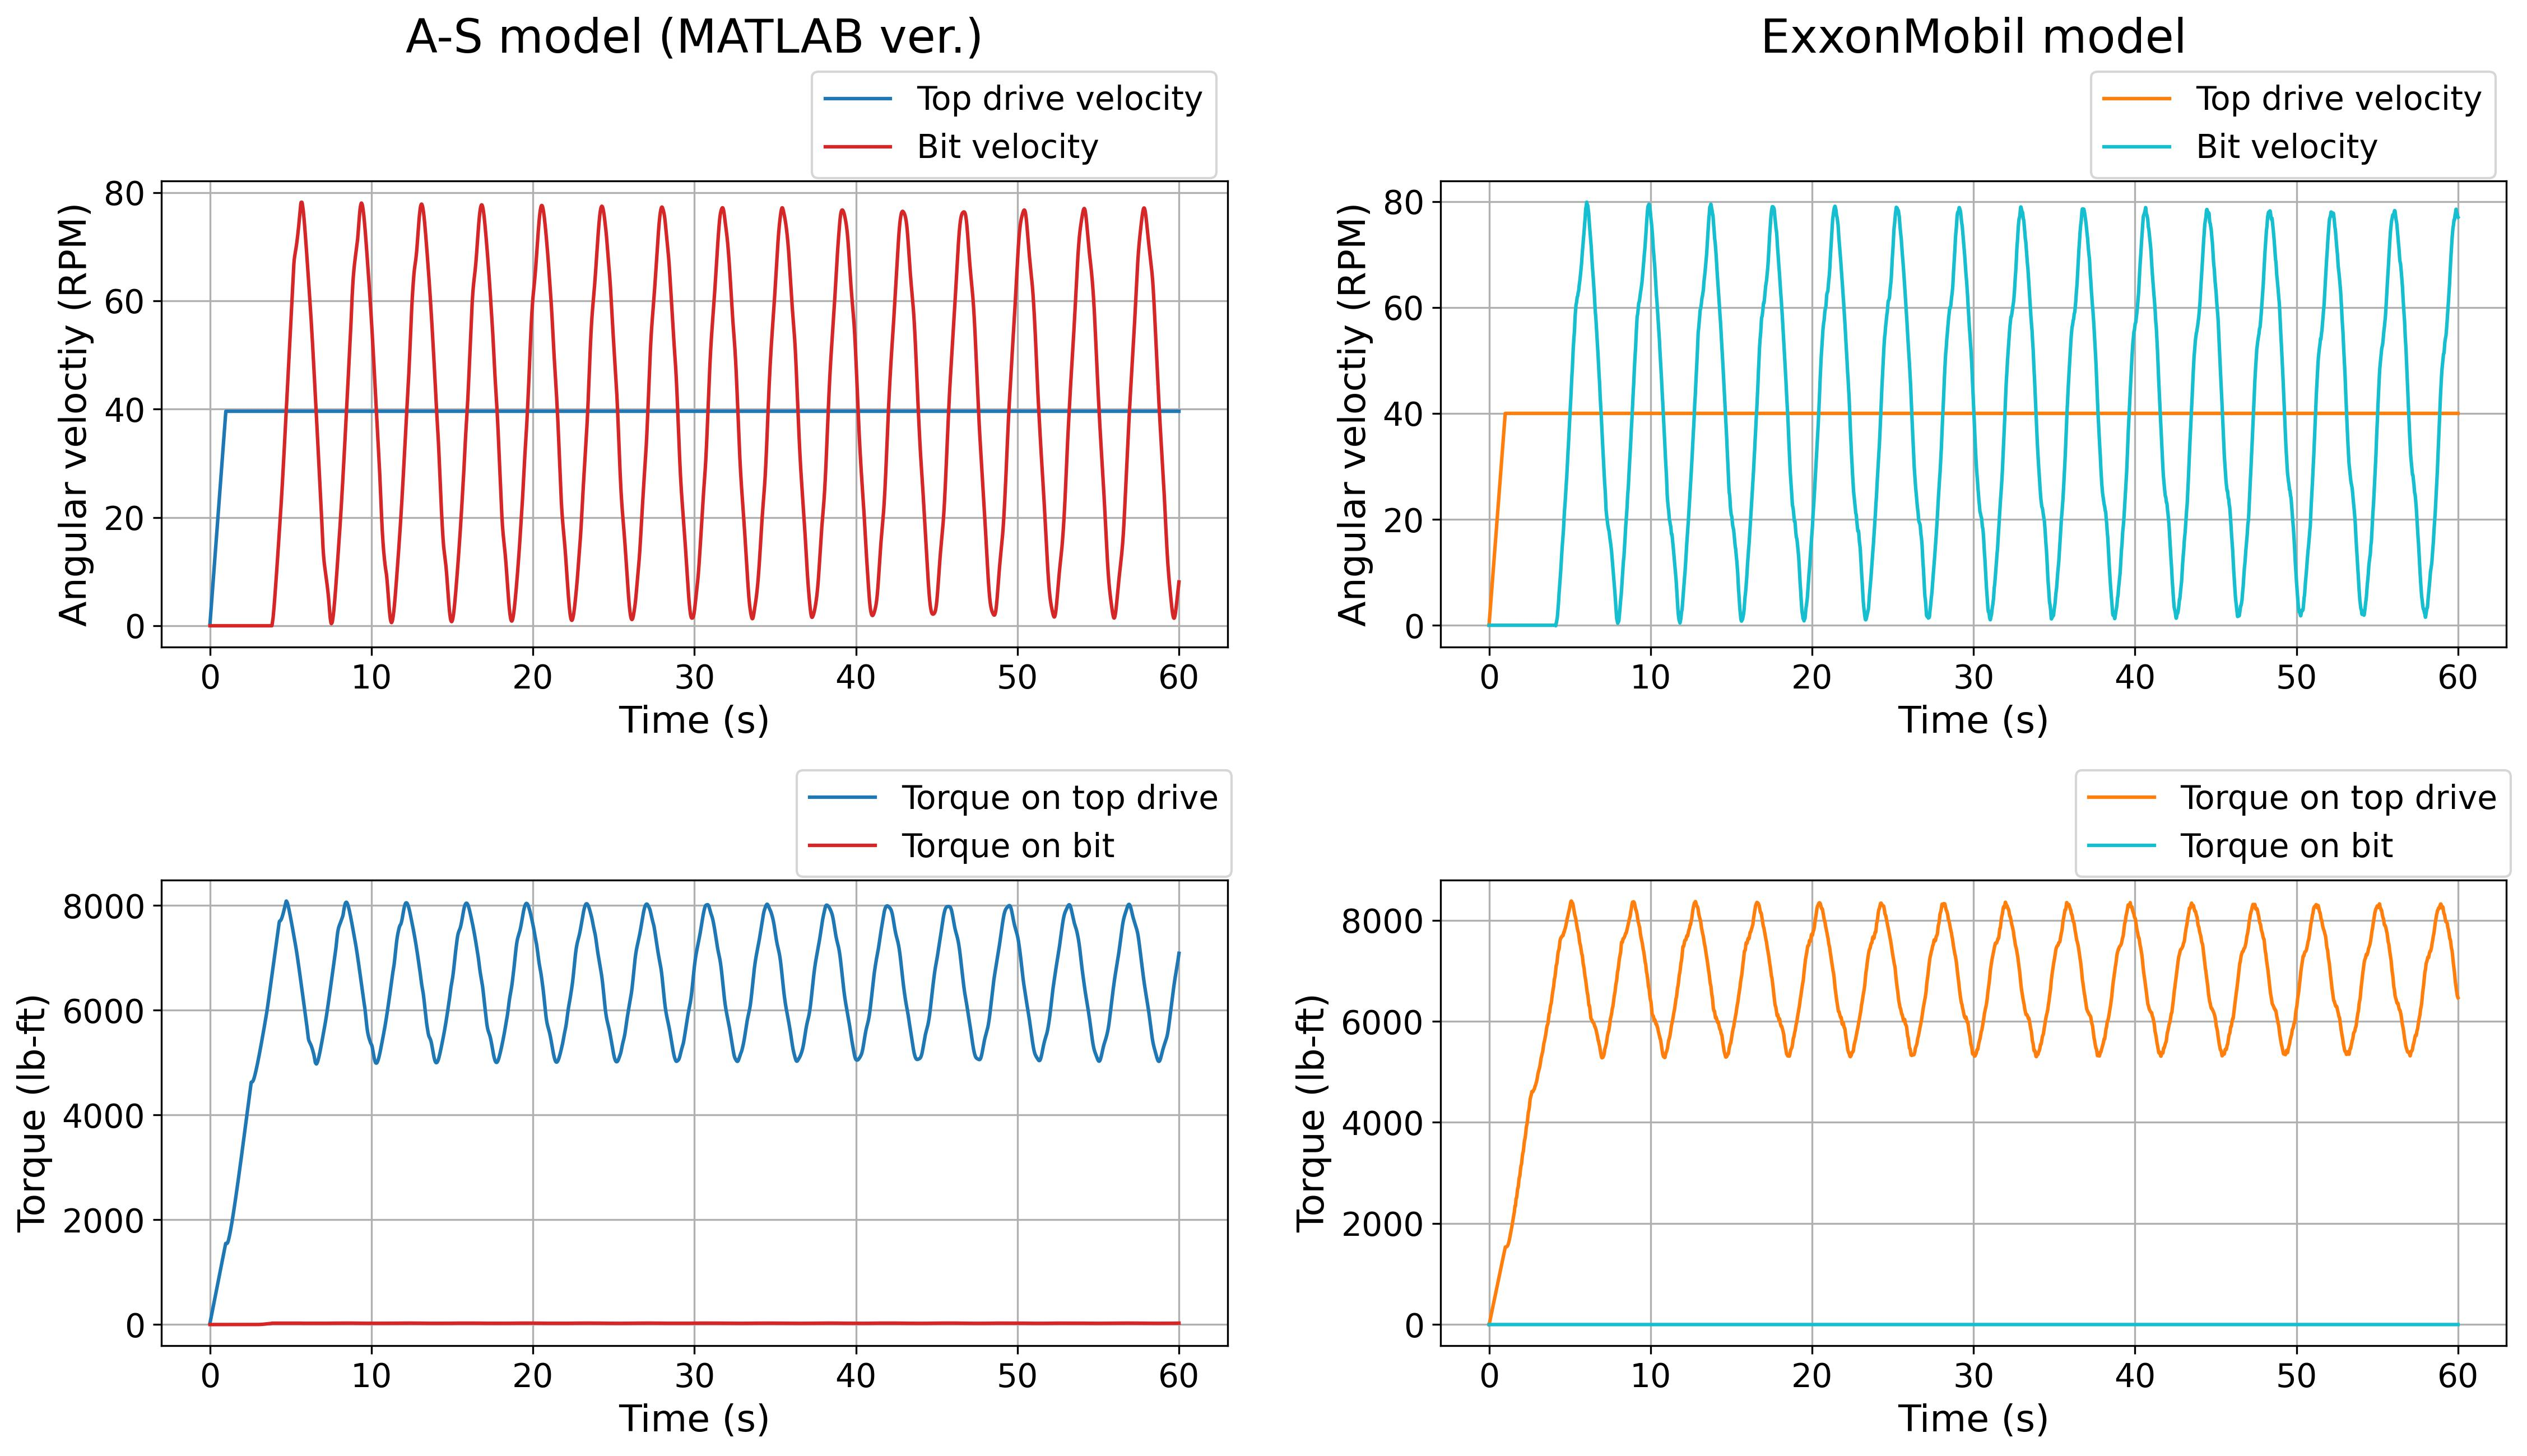
\includegraphics[width=6.5in]{output_figureTestCase4_1}
  \caption{}\label{figure_testcase4_1}
\end{figure}

\begin{figure}
  \centering
  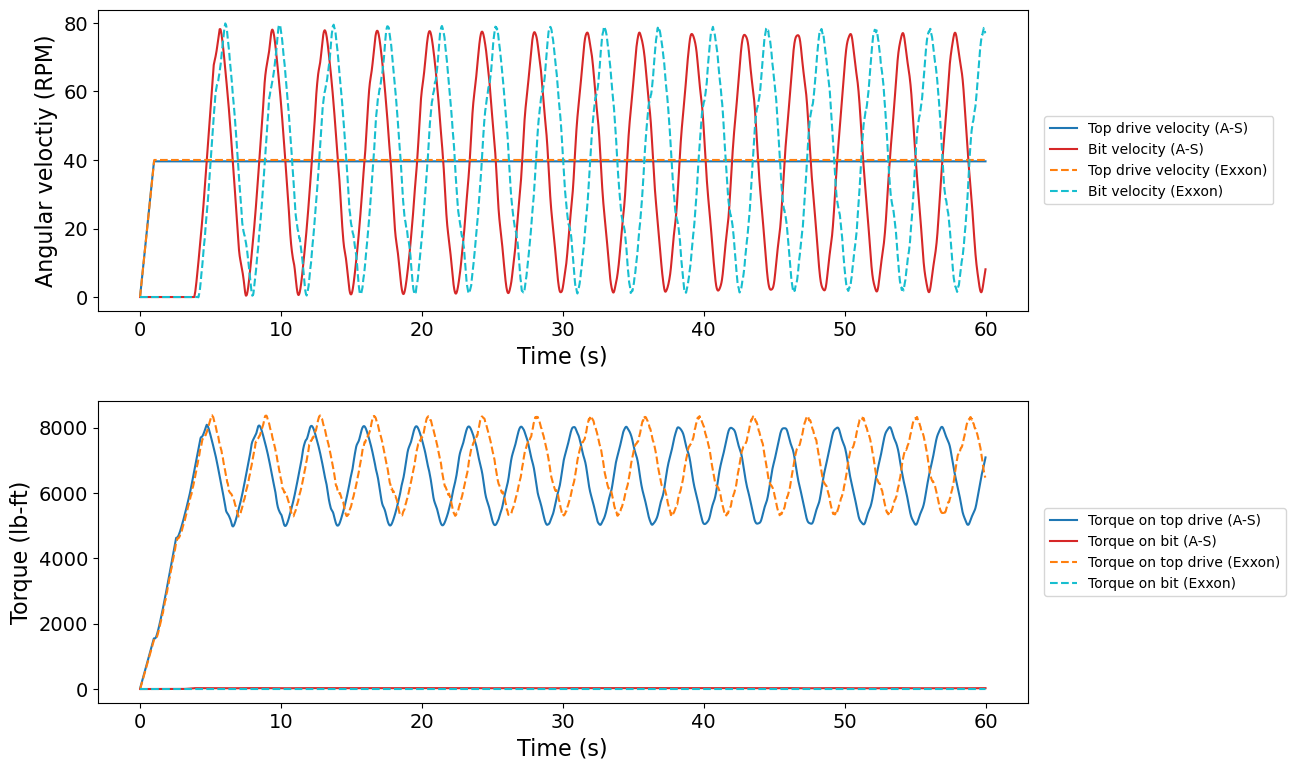
\includegraphics[width=6.5in]{overlapped_figureTestCase4_1}
  \caption{}\label{figure_testcase4_1_overlapped}
\end{figure}

\subsection{Test Case 4b}
\begin{figure}
  \centering
  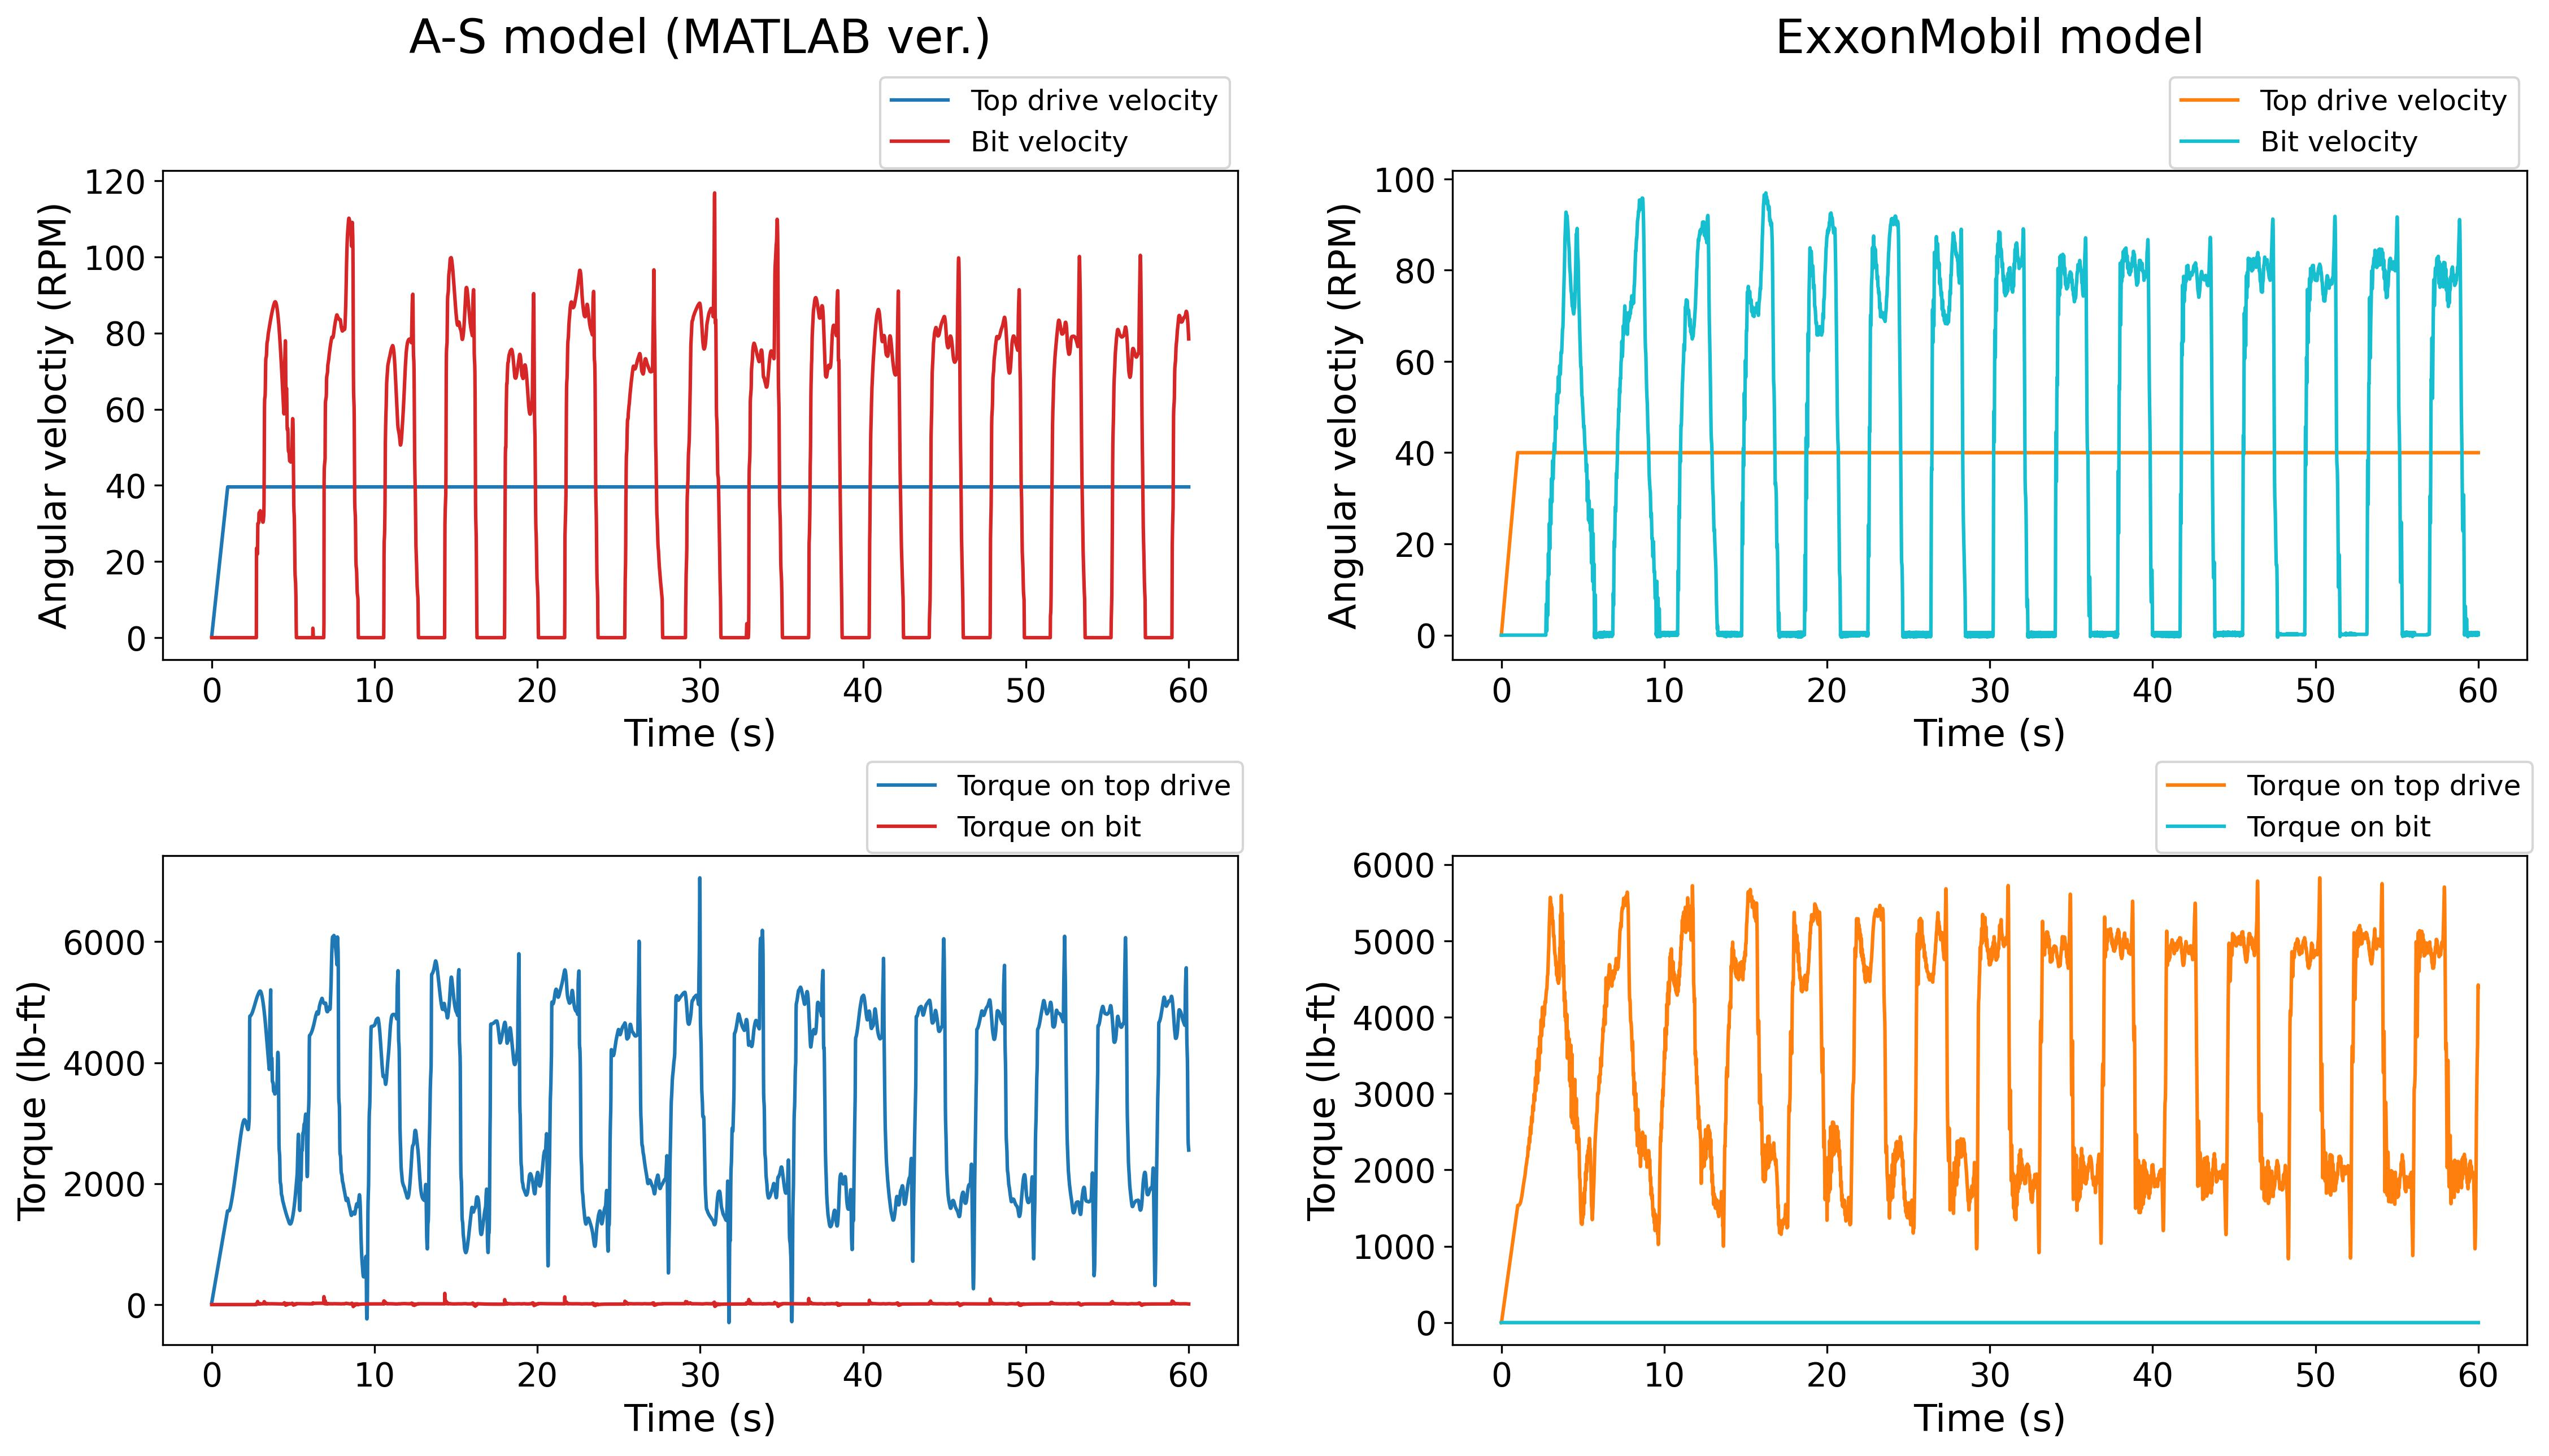
\includegraphics[width=6.5in]{output_figureTestCase4_2}
  \caption{}\label{figure_testcase4_2}
\end{figure}

\begin{figure}
  \centering
  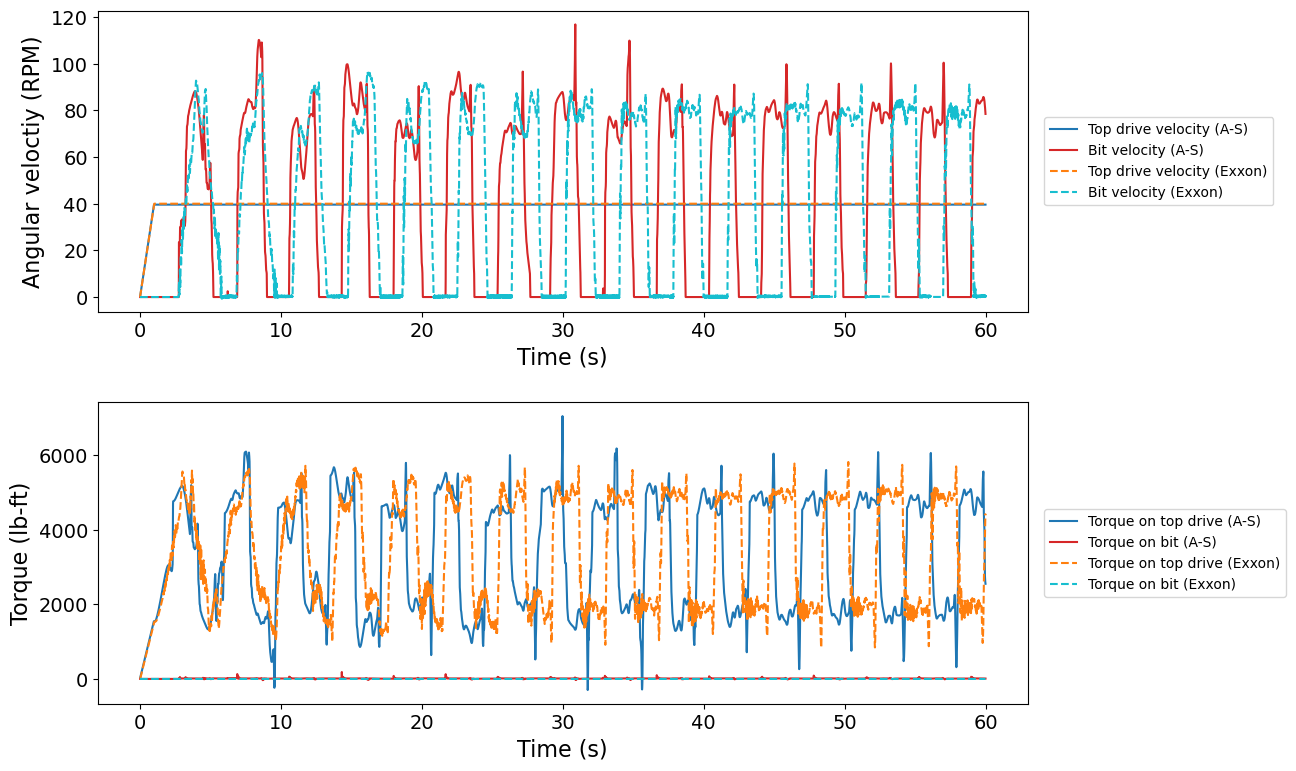
\includegraphics[width=6.5in]{overlapped_figureTestCase4_2}
  \caption{}\label{figure_testcase4_2_overlapped}
\end{figure}
